% Standalone LaTeX source. Bibliography, tables and plots are embedded.
% Compile twice with pdflatex. No external bibliography or figures are required.
\documentclass[11pt,a4paper]{article}
\usepackage[T1]{fontenc}
\usepackage[utf8]{inputenc}
\usepackage{lmodern}
\usepackage[margin=24mm,headheight=14pt]{geometry}
\usepackage{amsmath,amssymb,amsthm,bm,mathtools}
\usepackage{booktabs,array,tabularx,longtable}
\usepackage{graphicx,xcolor,microtype,enumitem,listings}
\usepackage{tikz,pgfplots}
\pgfplotsset{compat=1.18}
\usepackage{fancyhdr,placeins}
\usepackage[colorlinks=true,linkcolor=blue!45!black,citecolor=blue!45!black,
urlcolor=blue!45!black,pdftitle={WJ-EARSM neutral ASL and equilibrium-preserving analytical wall function}]{hyperref}
\usepackage[nameinlink,noabbrev]{cleveref}
\numberwithin{equation}{section}
\newtheorem{proposition}{Proposition}[section]
\newtheorem{remark}[proposition]{Remark}
\newcommand{\dd}{\mathrm d}
\newcommand{\eps}{\varepsilon}
\newcommand{\ust}{u_*}
\newcommand{\qe}{q_e}
\newcommand{\Ce}{C_*}
\newcommand{\ke}{\kappa_e}
\newcommand{\Ne}{N_e}
\newcommand{\tr}{\operatorname{tr}}
\newcommand{\diag}{\operatorname{diag}}
\newcommand{\I}{\mathsf I}
\newcommand{\R}{\mathsf R}
\newcommand{\units}[1]{\,\mathrm{#1}}
\newcommand{\pos}[1]{(#1)_+}
\setlength{\parindent}{0pt}
\setlength{\parskip}{4pt}
\setlength{\emergencystretch}{3em}
\setlist[itemize]{topsep=4pt,itemsep=2pt,parsep=0pt}
\setlist[enumerate]{topsep=4pt,itemsep=3pt,parsep=0pt}
\pagestyle{fancy}
\fancyhf{}
\fancyhead[L]{\small WJ-EARSM neutral ASL and analytical wall functions}
\fancyhead[R]{\small Research note}
\fancyfoot[C]{\thepage}
\lstdefinestyle{py}{language=Python,basicstyle=\ttfamily\scriptsize,
keywordstyle=\color{blue!55!black},commentstyle=\color{black!55},
stringstyle=\color{green!35!black},showstringspaces=false,
breaklines=true,columns=fullflexible,keepspaces=true,
frame=single,rulecolor=\color{black!20},framerule=0.3pt}
\title{\bfseries An analytical neutral atmospheric surface layer for the\\
Wallin--Johansson explicit algebraic Reynolds-stress model\\[4pt]
\large An equilibrium-preserving analytical wall function,\\
spectral/$hp$ coupling, curved terrain and stability}
\author{Standalone research note}
\date{10 November 2026}
\begin{document}
\maketitle
\begin{abstract}
The high-Reynolds-number Wallin--Johansson explicit algebraic
Reynolds-stress model (WJ-EARSM), with the $k$--$\eps$ completion used in
atmospheric wake modeling, admits a constant-stress logarithmic neutral
surface layer. Exact coefficient consistency gives
$C_*=572/6561$, $k_0=3.3867801405u_*^2$ and
$\kappa_e=0.3819178635$ when the scalar diffusivity uses $C_d=C_*$.
An analytical wall layer retains positive molecular viscosity, imposes
numerical no slip, and transfers total traction to this high-Re outer
flow. Its viscosity and dissipation coefficients are calibrated
simultaneously. A positive budget-matched dissipation profile and a
conservative redistribution preserve constant inner kinetic energy in
every spectral/$hp$ test mode. Curved normal coordinates supply mass,
momentum, scalar transport and conservative matching, including the
mechanical-pressure offset implied by anisotropic outer normal stress.

The constitutive assessment separates realizability, production and
incremental ellipticity. An exact rational certificate establishes a
positive incompressible principal bound $0.004\nu_{t,0}^{\rm eff}$ at
the neutral reference. This margin is local: an explicit simple-shear
state with normalized shear $q=3.5$ has negative oblique incremental
diffusion although its covariance is positive definite and production
is positive. The three-dimensional cubic-root approximation also has
an exact unrealizable counterexample. A separate sampled-$K$
destruction can drive local inner $k$ negative. Explicit optional
safeguards, their limits, and a staged validation programme are given.
The companion budget-cutoff appendix preserves the same outer reference
using nonconstant inner $k$ and ordinary diffusion instead of the EP
redistribution. Numerical checks verify the derived kernels and
certificates; they do not establish a native solver implementation or
validated terrain-flow predictions.
\end{abstract}

\textbf{Selected formulation.}
The default outer law is the three-dimensional explicit formula and
cubic $N$ approximation of Baungaard et al.\ \cite{Baungaard2022}.
The planar reduction is exact. Molecular viscosity is omitted only in
the declared high-Re outer equations; it is retained in all wall-layer
momentum, production, scalar diffusion, cutoffs and energy identities.
The default auxiliary coefficients are WJ-equilibrium calibrated.
Alternative roots, coefficient sets and robustness changes are named
explicitly instead of being silently mixed.

\clearpage
{\small\setlength{\parskip}{0pt}\tableofcontents}
\newpage

\section{Problem, notation and scope}
\label{sec:scope}
The objective is an outer neutral atmospheric surface layer (ASL) that
remains horizontally homogeneous over flat terrain, joined to a rough
analytical wall function (AWF) retaining explicit pressure-gradient
response. The constitutive model is due to Wallin and Johansson
\cite{WJ2000}; the high-Re atmospheric $k$--$\eps$ completion follows
Baungaard et al.\ \cite{Baungaard2022}; the underlying scalar rough-wall
kernel is due to Suga, Craft and Iacovides \cite{SCI2006}.
All subsequent equilibrium corrections and high-order coupling choices
are defined in this note.

\subsection{Coordinates, fields and reference notation}
Use Cartesian $(x,y,z)$, with $x$ streamwise, $y$ transverse and $z$
vertical. All tensor matrices use that order. The flat numerical ground
is $z=0$, and $0<z<H$ is a modeled wall layer, not a resolved viscous
sublayer. The outer domain is $H<z<Z$. The matching height $H$ is not
the ABL depth $Z$; the sand-grain roughness $h$ is not the aerodynamic
logarithmic intercept $z_0$. Curved surfaces use a separate physical
normal distance $r$ while $z$ remains Cartesian height.

Let $\bm U=(U,V,W)$, $\rho$ be constant density, $p$ mechanical pressure,
$\nu>0$ molecular kinematic viscosity, and
$R_{ij}=\overline{u_i'u_j'}$ the Reynolds covariance. Then
$k=\tfrac12R_{ii}$ and $\eps$ is the modeled dissipation of $k$.
The selected high-Re formulation transports this $\eps$ directly;
no modified-dissipation variable or extra length-scale source is
introduced. The mean gradient is $G_{ij}=\partial_jU_i$, and
$D/Dt=\partial_t+U_j\partial_j$. A prime on a mean profile means
ordinary differentiation with respect to its displayed height.

A subscript $0$ means evaluation on the selected reference, not
evaluation at the wall. The outer reference has
$\bm U_0=U_0(z)\bm e_x$, $k_0(z)=K_0>0$, and $\eps_0(z)>0$.
The current wall input is the endpoint trace
$K=k_w(H)=k_o(H)>0$; at the reference $K=K_0$.
Quantities $N_e,q_e,C_*,\kappa_e$ are equilibrium model constants.
The physical reference friction velocity is $u_*>0$ and
$t_0=\tau_{w,0}/\rho=u_*^2$.
The molecular parameter is always $\nu$; $\nu_{t,0}$ denotes an
eddy viscosity and is not a second molecular viscosity.

Three viscosities must be distinguished:
\begin{equation}
 \nu_t^{\rm eff}=C_\mu^{\rm eff}\frac{k^2}{\eps},
 \qquad \nu_d=C_d\frac{k^2}{\eps},
 \qquad \nu_{t,A}\quad\hbox{in the auxiliary wall model}.
 \label{eq:three-viscosities}
\end{equation}
The first belongs to the stress split, the second to scalar diffusion,
and the third is a prescribed wall-layer profile. They agree neither
in general flow nor at a finite wall/outer matching height.

\subsection{Equation domains and meaning of preservation}
The reference assumptions are incompressibility, neutral stratification,
zero mean system rotation, zero streamwise pressure gradient, and
horizontal homogeneity. Hydrostatic pressure can be retained and
subtracted exactly. The target is the constant-stress ASL, not a
logarithm throughout a finite pressure-driven or rotating ABL.

The selected composite model has:
\begin{enumerate}
\item outer high-Re WJ stress and $k$--$\eps$ equations;
\item finite-$\nu$ inner AWF momentum, retained inner $k$ transport,
and dependent inner dissipation;
\item matching mass, full traction and $k$ flux, with one prescribed
outer $\eps$ trace from the inner closure.
\end{enumerate}
No inner $\eps$ transport equation is claimed. Physical wall-layer
storage is retained in the curved/unsteady completion; independent
analytic columns are its flat quasi-steady reduction.

We distinguish an exact continuum reference, its finite-dimensional
projection, and a stationary fully discrete timestep. Success at the
first level does not prove the latter two. Positivity of a prescribed
rate, positivity of transported scalars, positive covariance and
positive incremental diffusion are also separate properties.

\section{The high-Reynolds-number WJ-EARSM}
\label{sec:wj-model}
\subsection{Tensor conventions and the explicit constitutive law}
Use the normalization of \cite{WJ2000,Baungaard2022}:
\begin{equation}
 \bm a=\bm R/k-\tfrac23\bm I,\qquad \tau=k/\eps,\qquad
 \bm S=\tfrac{\tau}{2}(\bm G+\bm G^T),\qquad
 \bm\Omega=\tfrac{\tau}{2}(\bm G-\bm G^T).
 \label{eq:wj-normalization}
\end{equation}
Incompressibility gives $\tr\bm S=0$. In particular this anisotropy
is twice the convention $\bm R/(2k)-\bm I/3$.
Define
\begin{equation}
 I_S=\tr\bm S^2\geq0,\quad I_\Omega=\tr\bm\Omega^2\leq0,\quad
 I_4=\tr(\bm S\bm\Omega^2),\quad
 I_5=\tr(\bm S^2\bm\Omega^2).
 \label{eq:wj-invariants}
\end{equation}
Here $I_4$ and $I_5$ correspond to the invariants denoted $IV,V$
in the original tensor formulation.

For $c_2=5/9$ set $c_1'=\tfrac94(c_1-1)>0$ and determine $N$
from the positive physical root of
\begin{equation}
 F(N):=N^3-c_1'N^2-
       \left(\tfrac{27}{10}I_S+2I_\Omega\right)N
       +2c_1'I_\Omega=0.
 \label{eq:wj-cubic}
\end{equation}
This specification avoids ambiguities in printed radical formulas.
For $N>0$, the equation is equivalent to
$(N-c_1')(N^2-2I_\Omega)=\tfrac{27}{10}NI_S$.
Thus its physical root obeys $N\geq c_1'$. On that interval,
$F(N)/N=N^2-c_1'N-2I_\Omega+
2c_1'I_\Omega/N-\tfrac{27}{10}I_S$ is strictly increasing because
$2N-c_1'-2c_1'I_\Omega/N^2>0$.
There is exactly one such positive root, and it is smooth in the
invariants. A bracketed scalar solve or a verified stable cubic
formula may be used.

For the selected three-dimensional law write
\begin{equation}
 \bm a=\beta_1\bm S+\beta_3\bm T_3+\beta_4\bm T_4
                   +\beta_6\bm T_6+\beta_9\bm T_9,
 \label{eq:wj-3d}
\end{equation}
where
\begin{align}
 \bm T_3&=\bm\Omega^2-\tfrac13I_\Omega\bm I,&
 \bm T_4&=\bm S\bm\Omega-\bm\Omega\bm S,\nonumber\\
 \bm T_6&=\bm S\bm\Omega^2+\bm\Omega^2\bm S-\tfrac23I_4\bm I,&
 \bm T_9&=\bm\Omega\bm S\bm\Omega^2-\bm\Omega^2\bm S\bm\Omega.
 \label{eq:wj-basis}
\end{align}
The coefficients are
\begin{equation}
 \begin{gathered}
 Q=\tfrac56(N^2-2I_\Omega)(2N^2-I_\Omega)>0,\\
 \beta_1=-\frac{N(2N^2-7I_\Omega)}Q,\quad
 \beta_3=-\frac{12I_4}{NQ},\quad
 \beta_4=-\frac{2(N^2-2I_\Omega)}Q,\quad
 \beta_6=-\frac{6N}Q,\quad \beta_9=\frac6Q.
 \end{gathered}
 \label{eq:wj-coefficients}
\end{equation}
This is the high-Re explicit model used in \cite{Baungaard2022}.
It gives a symmetric, tracefree $\bm a$; $\bm R=k(2\bm I/3+\bm a)$.
The useful positive implicit-viscosity split is
\begin{equation}
 C_\mu^{\rm eff}
 =-\tfrac12(\beta_1+I_\Omega\beta_6)
 =\frac{3N}{5(N^2-2I_\Omega)}>0.
 \label{eq:wj-ceff}
\end{equation}
The remaining tensor must still be included in momentum and production.
Positive \eqref{eq:wj-ceff} alone is not a full constitutive stability
certificate.

In a genuinely planar mean flow this reduces exactly to
\begin{equation}
 \bm a=-\frac{6N}{5(N^2-2I_\Omega)}\bm S
       -\frac{6}{5(N^2-2I_\Omega)}
          (\bm S\bm\Omega-\bm\Omega\bm S).
 \label{eq:wj-2d}
\end{equation}
The planar implicit ARSM identity is
$N=c_1'+\tfrac94\mathcal P/\eps$, where
$\mathcal P=-\eps\,\bm a:\bm S$.
The cubic root is an approximation to that identity in general
three-dimensional mean flow. Therefore a general implementation must
compute production from the full tensor; it must not substitute
$\mathcal P/\eps=4(N-c_1')/9$ outside its valid planar case.
The exact implicit three-dimensional alternative is discussed separately
in the stability assessment.

\subsection{Momentum and scalar transport}
The outer equations selected here are
\begin{align}
 \nabla\cdot\bm U_o&=0,\nonumber\\
 \partial_t\bm U_o+\nabla\cdot(\bm U_o\otimes\bm U_o)
 &=-\nabla(p_o/\rho)-\nabla\cdot\bm R_{\rm WJ}+\bm b,\label{eq:outer-momentum}\\
 \frac{Dk_o}{Dt}
 &=\mathcal P_o-\eps_o+
 \nabla\cdot\left(\frac{\nu_d}{\sigma_k}\nabla k_o\right),\label{eq:outer-k}\\
 \frac{D\eps_o}{Dt}
 &=(C_{\eps1}\mathcal P_o-C_{\eps2}\eps_o)\frac{\eps_o}{k_o}
 +\nabla\cdot\left(\frac{\nu_d}{\sigma_\eps}\nabla\eps_o\right),
 \quad \mathcal P_o=-\bm R_{\rm WJ}:\nabla\bm U_o.
 \label{eq:outer-epsilon}
\end{align}
Here $\bm b$ includes gravity if mechanical pressure is used.
Molecular diffusion is absent in these high-Re outer equations.
The finite value of $\nu$ is retained by the AWF below.
Scalar diffusion uses fixed $C_d$ in \eqref{eq:three-viscosities},
as in \cite[Section 2.4]{Baungaard2022}.
No near-wall damping, molecular timescale floor, buoyancy production,
system-rotation correction or extra dissipation source is selected.

The independent default coefficients are
\begin{equation}
 c_1=1.8,\quad c_2=5/9,\quad
 C_{\eps1}=1.44,\quad C_{\eps2}=1.82,\quad
 \sigma_k=1,\quad \sigma_\eps=1.30.
 \label{eq:default-constants}
\end{equation}
The chosen scalar coefficient $C_d=C_*$ and $\kappa_e$ are evaluated
from the exact equilibrium below. Their displayed decimal approximations
must not be independently rounded when testing exact identities.

\section{Derivation of the analytical neutral surface-layer reference}
\label{sec:outer-reference}
\subsection{Simple shear and the equilibrium branch}
For parallel shear define the scalar $G=U'(z)$ and $q=kG/\eps$;
the bold tensor $\bm G$ remains the full mean gradient. At the reference,
$\bm U_0=U_0(z)\bm e_x$ and $G_0=U_0'(z)>0$. Then
\begin{equation}
 \bm S=\frac q2
 \begin{pmatrix}0&0&1\\0&0&0\\1&0&0\end{pmatrix},\qquad
 \bm\Omega=\frac q2
 \begin{pmatrix}0&0&1\\0&0&0\\-1&0&0\end{pmatrix},
 \quad I_S=q^2/2,\quad I_\Omega=-q^2/2.
 \label{eq:simple-shear}
\end{equation}
The nonlinear tensor $\bm S\bm\Omega-\bm\Omega\bm S$
is $\tfrac12q^2\diag(-1,0,1)$.
Thus both selected planar and three-dimensional formulas give
\begin{equation}
 a_{xz}=-\frac{3Nq}{5(N^2+q^2)},\quad
 a_{xx}=\frac{3q^2}{5(N^2+q^2)},\quad
 a_{zz}=-a_{xx},\quad a_{yy}=0,\quad
 \frac{\mathcal P}{\eps}=C_\mu^{\rm eff}q^2.
 \label{eq:shear-stress}
\end{equation}
The cubic reduces to
$N^3-c_1'N^2-\tfrac7{20}q^2N-c_1'q^2=0$.
For constant reference $k_0=K_0$, its transport requires
$\mathcal P_{o,0}=\eps_0$, so
\begin{equation}
 \boxed{
 N_e=\tfrac94c_1,\quad
 q_e^2=\frac{N_e^2}{3N_e/5-1},\quad
 C_*=\frac1{q_e^2}=\frac{108c_1-80}{405c_1^2}.}
 \label{eq:equilibrium-constants}
\end{equation}
The selected $c_1=1.8$ gives
\begin{equation}
 N_e=\frac{81}{20},\qquad C_*=\frac{572}{6561},\qquad
 q_e=\frac{81}{2\sqrt{143}}=3.386780140528718.
 \label{eq:exact-root}
\end{equation}
$N$ is not frozen to $N_e$ away from the reference.

\subsection{Constant stress and dissipation-transport compatibility}
Require $R_{xz,0}=-u_*^2$. Since $a_{xz,e}=-1/q_e$, this fixes
$K_0=q_eu_*^2$. Production then fixes
$\eps_0=u_*^2G_0$. For a logarithm,
\begin{equation}
 \boxed{
 U_0(z)=\frac{u_*}{\kappa}\ln\frac z{z_0},\quad
 k_0=K_0=q_eu_*^2,\quad
 \eps_0(z)=\frac{u_*^3}{\kappa z},\quad
 \nu_{t,0}^{\rm eff}=\kappa u_*z.}
 \label{eq:outer-reference-family}
\end{equation}
Its stress is constant, and the momentum and $k$ equations vanish.
The scalar diffusivity is
$\nu_{d,0}=(C_d/C_*)\kappa u_*z$. Substitution into the
dissipation equation gives
\begin{align}
 \frac{\dd}{\dd z}
 \left(\frac{\nu_{d,0}}{\sigma_\eps}\eps_0'\right)
 &=\frac{C_d}{C_*}\frac{u_*^4}{\sigma_\eps z^2},\nonumber\\
 \mathcal R_{\eps,0}
 &=\left[C_{\eps1}-C_{\eps2}
 +\frac{C_d\kappa^2}{\sigma_\eps C_*^{3/2}}\right]\frac{\eps_0^2}{K_0}.
 \label{eq:epsilon-reference-residual}
\end{align}
Hence
\begin{equation}
 \boxed{\kappa^2
 =\sigma_\eps(C_{\eps2}-C_{\eps1})\frac{C_*^{3/2}}{C_d}.}
 \label{eq:kappa-compatibility}
\end{equation}
For $C_d=C_*$ this yields
\begin{equation}
 \boxed{\kappa_e
 =\sqrt{1.30(1.82-1.44)\sqrt{572/6561}}
 =0.381917863546733.}
 \label{eq:kappa-default}
\end{equation}
This derives the log-layer relation in
\cite[Equations (22)--(23)]{Baungaard2022}.
The molecular coefficient $\nu$ does not enter this outer derivation.

\subsection{Complete stress and pressure reference}
At equilibrium
\begin{equation}
 \frac{\bm R_0}{K_0}=
 \begin{pmatrix}
 2/3+1/N_e&0&-1/q_e\\
 0&2/3&0\\
 -1/q_e&0&2/3-1/N_e
 \end{pmatrix}.
 \label{eq:outer-covariance}
\end{equation}
The eigenvalues are
$2/3$ and $2/3\pm\sqrt{N_e^{-2}+C_*}$,
approximately $0.666666667$, $0.281766487$, and $1.051566846$.
The tensor is positive definite. Its normal components divided by
$u_*^2$ are $3.094095437$, $2.257853427$, and $1.421611417$.
In particular $R_{xz,0}=-u_*^2$ is nonzero.
All stresses are height-independent; reduced outer pressure is constant,
or $p_{o,0}'=-\rho g$ if physical hydrostatic pressure is retained.

\section{Relation to neutral Monin--Obukhov profiles and coefficient choices}
\label{sec:most}
The functional forms in \eqref{eq:outer-reference-family} are the neutral
constant-flux surface-layer forms. The closure determines their
$k/u_*^2$ ratio, anisotropy and compatible logarithmic slope. A logarithmic
velocity inlet alone is not an equilibrium specification.
The additive velocity offset is not fixed by the outer differential
equations; the wall coupling below fixes it and therefore the effective
$z_0$.

The printed atmospheric values $C_\mu=0.087$ and $\kappa=0.38$
are finite-precision presentations. Keeping $C_d=0.087$ literally while
using the exact constitutive $C_*$ gives
$\kappa=0.382316763868004$ from \eqref{eq:kappa-compatibility}.
The selected $C_d=C_*$ instead gives \eqref{eq:kappa-default}.
Using $0.087$ in the inlet $k$ and $0.38$ in the velocity and $\eps$
profiles gives $\mathcal P/\eps=1.001119195521694$, so it is only
an approximate equilibrium.

If a prescribed target $\kappa_t$ is required, a single transport
coefficient may be recalibrated:
\begin{equation}
 \sigma_\eps^{\,t}
 =\frac{C_d\kappa_t^2}
 {C_*^{3/2}(C_{\eps2}-C_{\eps1})},
 \quad\hbox{or}\quad
 C_{\eps1}^{\,t}
 =C_{\eps2}-\frac{C_d\kappa_t^2}{\sigma_\eps C_*^{3/2}}.
 \label{eq:target-kappa}
\end{equation}
For $\kappa_t=0.40$ and $C_d=C_*$ these are
$\sigma_\eps^{\,t}=1.426012690748934$ or
$C_{\eps1}^{\,t}=1.403165521165696$, respectively.
Use one change, not both. The former retains the homogeneous
source-only $k$--$\eps$ dynamics; the latter changes them.
Both change some off-reference predictions. The default in this note
keeps \eqref{eq:default-constants} and uses $\kappa_e$.
The wall coefficients must be recomputed if a different compatible
$\kappa$ is chosen.

Changing the stress coefficient $c_1$ is unnecessary for this goal.
It changes anisotropy, and $C_*(c_1)\leq0.09$ implies
$\kappa\leq0.3849675311$ when $C_d=C_*$ and the default transport
coefficients remain fixed. It cannot alone obtain $\kappa=0.40$.


\section{A calibrated analytical wall function}
\label{sec:wj-wall-kernel}

The outer model uses the high-Reynolds-number equations specified above.
Molecular momentum and scalar diffusion are omitted there, whereas the
physical molecular viscosity $\nu>0$ is retained throughout the modeled
wall layer. These are two declared equation systems joined by conservative
interface conditions. No assertion is made that an unshifted logarithm
solves the finite-Reynolds-number equations down to the numerical wall.

Use Cartesian coordinates $(x,y,z)$, with streamwise $x$ and vertical $z$.
For a flat surface the numerical ground is $z=0$, the physical matching
height is $H>0$, and the modeled wall layer is $0\leq z\leq H$.
The equivalent sand-grain roughness $h$ satisfies $0\leq h<H$; it differs
from the aerodynamic logarithmic intercept $z_0$. The selected sampling is
\begin{equation}
 K=k_w(H)=k_o(H)>0.
 \label{eq:wj-wall-K}
\end{equation}
The subscripts $w$ and $o$ denote inner and outer fields. A fixed interior
sample or a normalized average is a possible alternative, but it defines
a different wall model and must be specified independently of polynomial
degree or quadrature nodes. The chosen endpoint sample is used below.

The equilibrium constants are denoted by $q_e$, $C_*=q_e^{-2}$ and
$\kappa_e$. For every current positive sample $K$, define a counterfactual
zero-forcing reference family by
\begin{equation}
 u_*(K)=\sqrt{K/q_e},\qquad t_0(K)=K/q_e,\qquad
 A_e(K)=\frac{u_*(K)^3}{\kappa_e}.
 \label{eq:wj-wall-ref-scales}
\end{equation}
These quantities do not impose the actual traction in a developing flow.
All reference quantities appearing in one wall evaluation use the same
current $K$. One fixed inlet is obtained by choosing $K=K_0$.

\subsection{Published parameters and the selected calibration}

The rough-wall analytical model of Suga, Craft and Iacovides \cite{SCI2006} uses an
auxiliary viscosity
\begin{equation}
 z^*=z\sqrt K/\nu,\quad h^*=h\sqrt K/\nu,\quad
 \nu_{t,A}=\nu\max\{0,\alpha(z^*-b)\},\quad
 D_A=\nu+\nu_{t,A}>0,\quad \alpha=c_\mu^wc_\ell^w.
 \label{eq:wj-wall-viscosity}
\end{equation}
The superscript $w$ denotes auxiliary wall-model coefficients, not the
flow-dependent outer EARSM coefficient. The published set has
$(c_\mu^w,c_\ell^w,\alpha)=(0.09,2.55,0.2295)$. This note instead selects
the equilibrium-compatible set
\begin{equation}
 \boxed{c_\mu^w=C_*,\qquad c_\ell^w=\kappa_e q_e^{3/2},\qquad
 \alpha=\kappa_e/\sqrt{q_e}.}
 \label{eq:wj-wall-calibration}
\end{equation}
For the stated WJ transport constants these values are
\begin{equation}
 c_\mu^w=0.0871818320377991,\quad
 c_\ell^w=2.3804029452632984,\quad
 \alpha=0.2075278897562272.
\end{equation}
Writing $a=\alpha\sqrt K$, the calibration gives the useful identities
\begin{equation}
 \boxed{a=\kappa_e u_*,\qquad
 K^{3/2}/c_\ell^w=A_e=t_0^2/a.}
 \label{eq:wj-wall-calibration-identities}
\end{equation}
Thus the dissipation tail coefficient and the asymptotic viscosity slope
both match the outer equilibrium. Their matching is a new calibration;
it does not preserve every published numerical rough-wall prediction.
The mathematical EP construction below also works with the published
coefficient set, provided all integrals and its distinct baseline are
recomputed. Choosing a different prescribed $\kappa$ first requires a
compatible outer transport model, followed by the corresponding wall
calibration. Merely replacing $\kappa_e$ in the wall coefficients cannot
repair an incompatible outer dissipation equation.

Retain the published roughness-intercept correlation. For $h^*>0$ set
\begin{equation}
 \begin{aligned}
 b&=10.7\left[1-(h^*/70)^m\right],\\
 m&=\max\left\{0.5-0.4(h^*/70)^{0.7},
                 1-0.79(h^*/70)^{-0.28}\right\}.
 \end{aligned}
 \label{eq:wj-wall-roughness}
\end{equation}
For $h=0$ use $b=10.7$ directly. With $z_v=\nu b/\sqrt K$,
$\nu_{t,A}=a\max(z-z_v,0)$. Negative $z_v$ is the virtual intercept
of a viscosity line; it is not clipped to zero or interpreted as a
negative physical distance. Retaining this empirical correlation while
changing the viscosity slope does not independently preserve a measured
aerodynamic roughness.

The adapted original-cutoff dissipation is one continuous positive field,
\begin{equation}
 \boxed{E_A(z)=\frac{A_A}{\max(z,z_{\varepsilon,A})},\qquad
 A_A=K^{3/2}/c_\ell^w,\qquad
 z_{\varepsilon,A}=2c_\ell^w\nu/\sqrt K.}
 \label{eq:wj-wall-original-E}
\end{equation}
Indeed, $A_A/z_{\varepsilon,A}=2\nu K/z_{\varepsilon,A}^2$.
The dimensionless cutoff is $2c_\ell^w$, which equals
$4.760805890526597$ for the selected calibration, rather than the
published value $5.1$. The viscosity intercept and this dissipation
cutoff are distinct. For the selected calibration $A_A=A_e$.

\subsection{Momentum, production and signs}

In the flat quasi-steady reduction, a sampled tangential acceleration
$\bm F=\bm F_a+\bm F_p$ is constant above $h$ and suppressed below it.
For mechanical pressure $\bm F_p=\rho^{-1}\nabla_\parallel p$; any
gravity or reduced-pressure convention must be included consistently.
Define
\begin{equation}
 L_h(z)=(z-h)_+,\quad
 J_0(z)=\int_0^z\frac{ds}{D_A(s)},\quad
 J_1(z)=\int_0^z\frac{L_h(s)}{D_A(s)}\,ds,\quad
 J_2(z)=\int_0^zD_A(s)^{-2}\,ds.
 \label{eq:wj-wall-integrals}
\end{equation}
An omitted argument means evaluation at $H$ and $B=J_1/J_0$.
The solution of $(D_A\bm U_A')'=\bm F\,\mathbf1_{z>h}$ with
$\bm U_A(0)=0$ and $\bm U_A(H)=\bm U_H$ is
\begin{equation}
 \boxed{\begin{aligned}
 \bm t_A&=\bm U_H/J_0-B\bm F,\\
 \bm U_A(z)&=\bm t_AJ_0(z)+\bm FJ_1(z),\\
 D_A\bm U_A'&=\bm t_A+\bm F L_h(z),\\
 \bm T_H&=\bm t_A+\bm F(H-h).
 \end{aligned}}
 \label{eq:wj-wall-momentum}
\end{equation}
$\bm t_A$ is the shear in the upward gradient-flux convention. The force
of the ground on the fluid has the opposite sign. Reversed shear remains
signed. The outer domain's lower normal is $-\bm e_z$, so its tangential
stress load is $-\rho\bm T_H$, not $-\rho\bm t_A$ when forcing is present.
Production and its mean are
\begin{equation}
 P_A(z)=\nu_{t,A}\left|\frac{\bm t_A+\bm F L_h}{D_A}\right|^2,
 \qquad \overline P_A=H^{-1}\int_0^H P_A\,dz.
 \label{eq:wj-wall-production}
\end{equation}
At fixed $K,h,H,\nu,\bm U_H$, the exact reduced-kernel response is
$\partial\bm t_A/\partial\bm F=-B I_T$ and
$\partial\bm T_H/\partial\bm F=(H-h-B)I_T$.
The calibration changes their numerical values but retains their form.


\section{Free velocity anchor and one common EP dissipation field}
\label{sec:wj-wall-ep}

Choose the outer free velocity offset through
\begin{equation}
 U_{H,0}=t_0J_0(H),\qquad
 U_{o,0}(z)=t_0J_0(H)+\frac{u_*}{\kappa_e}\ln\frac zH,
 \qquad z_0=H\exp[-\kappa_e u_*J_0(H)].
 \label{eq:wj-wall-anchor}
\end{equation}
The inner reference is $U_{w,0}=t_0J_0(z)$ and satisfies numerical
no slip. At the matching surface,
$D_A(H)U_{w,0}'(H)=\nu_{t,o,0}(H)U_{o,0}'(H)=t_0$.
Continuity of derivatives is not required because the constitutive
diffusivities differ. The logarithm is used only for $z\geq H$.
For fixed $u_*,h,H,\nu$, the intercept is an output. An independently
specified $z_0$ requires an additional momentum/intercept calibration.
In an FV implementation with an interpolated matching value, the free
offset must instead satisfy the actual discrete interpolation equation;
an exact continuum value at $H$ cannot be substituted for that operation.

On the fully active rough branch $z_v\leq0$, set $d=\nu-az_v\geq\nu$.
Then
\begin{equation}
 \begin{gathered}
 D_A=d+az,\qquad J_0(H)=a^{-1}\ln(1+aH/d),\\
 J_2(H)=a^{-1}[d^{-1}-(d+aH)^{-1}],\qquad
 \boxed{z_0=\frac{dH}{d+aH}.}
 \end{gathered}
 \label{eq:wj-wall-rough-anchor}
\end{equation}
Even with matching asymptotic slopes the intercept has a finite-$H$
dependence; it approaches $d/a$ only when $aH\gg d$. If a separately
prescribed $0<z_0<H$ is required, this linear-branch momentum calibration
would demand $d=aHz_0/(H-z_0)$, subject to its branch condition. It
generally cannot also retain an independently fixed empirical $b(h^*)$
and $h$. A dissipation-only correction cannot supply that extra freedom.

The counterfactual pointwise production and budget are
\begin{equation}
 \boxed{p_{A,0}(z)=t_0^2\frac{\nu_{t,A}}{D_A^2},\qquad
 \mathcal P_0=H\overline P_0=\int_0^H p_{A,0}\,dz
 =t_0^2(J_0-\nu J_2).}
 \label{eq:wj-wall-budget}
\end{equation}
The nonnegative integral is preferable to cancellation of $J_0-\nu J_2$
near a molecular branch. Neither $p_{A,0}$ nor $\overline P_0$ is the
current forced production. Replacing the reference budget by the current
production would suppress the intended non-equilibrium source response.

Choose a physical tail-start height $0<z_m\leq H$ and define
\begin{equation}
 E_c(z)=\frac{A_e}{\max(z,z_c)},\qquad
 \Lambda=\frac{\mathcal P_0}{A_e},\qquad
 \boxed{z_c=H\exp(1-\Lambda).}
 \label{eq:wj-wall-cutoff}
\end{equation}
The corrected profile is finite, positive, continuous and nonincreasing.
Its mean equals $\overline P_0$ because
\begin{equation}
 \int_0^H E_c\,dz=A_e[1+\ln(H/z_c)]=\mathcal P_0.
 \label{eq:wj-wall-cutoff-budget}
\end{equation}
The necessary and sufficient monotone-tail gate is
\begin{equation}
 \boxed{z_c\leq z_m\quad\Longleftrightarrow\quad
 \Lambda\geq1+\ln(H/z_m).}
 \label{eq:wj-wall-cutoff-gate}
\end{equation}
To see necessity, any nonnegative nonincreasing continuation that equals
$A_e/z$ for $z\geq z_m$ has an integral at least
$A_e[1+\ln(H/z_m)]$. The displayed cap realizes every greater budget.
Equivalently $z_c=z_m\exp[1+\ln(H/z_m)-\Lambda]$; the factor $H$ in
the simpler expression cannot be replaced by $z_m$ alone. A failed gate
is not repaired by clipping $z_c$, since clipping changes the budget.
Endpoint matching requires only $z_m=H$; this note's numerical example
uses the stronger $z_m=H/2$.

For $0\leq\chi\leq1$, constant along a wall-normal ray, use one blend
\begin{equation}
 E_{\rm pre}=(1-\chi)E_A+\chi E_c.
 \label{eq:wj-wall-blend}
\end{equation}
Its mean, any selected point sample, and the outer dissipation trace
are obtained from this same field. In particular,
$\varepsilon_o(H)=E_{\rm pre}(H)$ before the positivity amendment below.
Inner dissipation is dependent; no independent inner dissipation PDE or
additional prescribed interface dissipation flux is imposed. When a
first FV dissipation value is constrained instead, its algebraic row
must replace, rather than supplement, an independent transport row.

The reference mean kinetic-energy balance is
\begin{equation}
 t_0U_{H,0}=\mathcal P_0+\nu t_0^2J_2
 =\int_0^H E_c\,dz+\nu\int_0^H(U_{w,0}')^2\,dz.
 \label{eq:wj-wall-energy}
\end{equation}
The stationary no-slip ground does no work; the left side is the power
entering the layer through its upper matching surface.
Combining the anchor and budget also gives
$z_c=e z_0\exp(\kappa_e u_*\nu J_2)$; on the calibrated linear rough
branch the last exponent is $\nu[d^{-1}-(d+aH)^{-1}]$. The budget
cutoff is therefore distinct from both a molecular cutoff and a
measured roughness length, even when their asymptotic scales are related.


\section{Properties of the proposed wall closure}
\label{sec:wall-properties}
\subsection{Exact reference, no slip and interface flux}
The composite EP reference uses $U_{w,0}=t_0J_0(z)$ below $H$,
the anchored logarithm above $H$, constant $k=K_0$ throughout, and
$E_c$ below $H$ with $\eps_0=A_e/z$ above it. The outer equations
vanish by \cref{sec:outer-reference}. The wall momentum reconstruction
satisfies its finite-$\nu$ differential equation and exact ground
no slip. Its interface value and total tangential traction agree with
the outer state. The integrated $k$ budget follows from the cutoff;
pointwise wall $k$ balance in a high-order retained layer additionally
requires the redistribution in \cref{sec:wj-wall-moments}.
The normal-pressure offset derived in \cref{sec:wj-wall-curved}
completes the momentum equilibrium.

These are statements about the composite field. Applying the outer
logarithm inside the modeled wall layer instead would change the
target. Neither $U_{w,0}'(H)=U_{o,0}'(H)$ nor continuity of
$\nu_{t,A}$ with $\nu_{t,o}^{\rm eff}$ is required.
At fixed $K,\bm F,H,h,\nu$, the condensed interface coefficient is
$\partial\bm T_H/\partial\bm U_H=J_0^{-1}I_T>0$.
That frozen scalar positivity does not certify the outer nonlinear
stress tangent or the coupled pressure problem.

\subsection{Mechanical power and molecular loss}
Multiplication of the scalar AWF momentum equation by $U_A$ gives
\begin{equation}
 T_HU_H=\int_0^H D_A(U_A')^2\,dz
              +F\int_h^H U_A\,dz.
 \label{eq:forced-wall-power}
\end{equation}
For the vector tangential problem replace products by dot products.
The last term is the work associated with the sampled pressure and
convective forcing in this reduced balance; it is not a separately
guaranteed positive loss. At zero forcing,
\begin{equation}
 t_0U_{H,0}
 =\nu t_0^2J_2+\int_0^Hp_{A,0}\,dz
 =\nu\int_0^H(U_{w,0}')^2\,dz+\int_0^HE_c\,dz.
 \label{eq:wall-power-reference}
\end{equation}
The molecular term must not be discarded or folded into turbulent
production. Keeping $\nu$ in $D_A$ but using $D_A(U_A')^2$ as turbulent
production would double count this loss.

\subsection{Pressure-gradient response and recovery}
At frozen $K,U_H,h,H,\nu$, put
$g_F(z)=[L_h(z)-B]/D_A(z)$. For a scalar forcing component,
\begin{equation}
 U_A'=U_H/[J_0D_A]+Fg_F,\qquad
 \partial_F\overline P_A
 =\frac2H\int_0^H\nu_{t,A}U_A'g_F\,dz,\qquad
 \partial_F^2\overline P_A
 =\frac2H\int_0^H\nu_{t,A}g_F^2\,dz\geq0.
 \label{eq:wall-pressure-response}
\end{equation}
The EP dissipation is built from the counterfactual zero-forcing
reference, not from current $\overline P_A$. At fixed $\chi$ its mean
source therefore has exactly the baseline production response.
Derivatives of an evolving $\chi$ and $K$ remain part of the coupled
operator. A plateau switch retains this frozen response in a
neighborhood of the reference.

At $\chi=0$ the selected calibrated original-cutoff kernel is recovered.
This means recovery with the same $K,U_H,F,H,h,\nu$ and coefficient set.
It does not mean recovery of the historical numerical parameter values
after changing $c_\mu^w,c_\ell^w$, or equivalence of solutions with
different upstream histories. The high-order and curved representations
also remain part of the adapted baseline.

\section{Equilibrium activation and admissibility}
\label{sec:activation}
The correction is useful only where a specified undisturbed reference
should be preserved. Its weight is ray-constant, $0\leq\chi\leq1$.
Reference samples, not arbitrary local production, define the target.
Useful dimensionless residual sensors are, for example,
\begin{equation}
 \begin{aligned}
 r_U&=(U_H-t_0J_0)/u_s,&
 r_{\Delta U}&=[U(z_b)-U(z_a)
            -(u_*/\kappa_e)\ln(z_b/z_a)]/u_s,\\
 r_k&=[k(z_b)-k(z_a)]/K_s,&
 r_\eps&=[\eps(z_b)-A_e/z_b]/\eps_s,\\
 r_p&=HF_p/u_s^2,&
 r_a&=HF_a/u_s^2,\qquad r_W=W_H/u_s ,
 \end{aligned}
 \label{eq:reference-sensors}
\end{equation}
where $z_a,z_b\geq H$ are fixed outer evaluation heights and
$u_s,K_s,\eps_s>0$ are declared normalization scales.
The $\eps$ sensor must use an independent outer unknown, not the
algebraically imposed trace. Separate $F_p,F_a$ prevent their sum from
concealing large mutually cancelling terms. In a discrete scheme all
reference values in these sensors are evaluated with the same operators
as current data.

For any positive weights $\omega_j$, use
$r^2=\sum_j\omega_jr_j^2$ and a gate equal to one for
$r\leq r_{\rm on}$, equal to zero for $r\geq r_{\rm off}>r_{\rm on}$,
and $1-10s^3+15s^4-6s^5$ in between, where
$s=(r-r_{\rm on})/(r_{\rm off}-r_{\rm on})$.
The thresholds are declared model inputs; no universal calibration is
asserted. The exact unit plateau is important for preservation of both
the reference and its linearized wall-source response.

Admissibility additionally requires $K>0$, $\nu>0$, $0\leq h<H$,
an invertible wall geometry and the cutoff gate. The correction must
vanish strictly before a failed gate is evaluated. At $\chi=0$ evaluate
the baseline directly, without computing an invalid $E_c$ first.
Clipping $z_c$ to a matching height destroys the exact budget.
If the intended reference itself violates the gate, it is outside this
construction and no preservation claim is made. Changing $H$, the
physical roughness or the chosen monotone continuation is a model change.

\section{Finite-volume comparison and discrete preservation}
\label{sec:fv}
In a cell-centered FV realization the first cell occupies $[0,H]$,
has center $P$ at $z_P$, and obtains $U_H$ from a declared interpolation
of adjacent resolved values. That auxiliary input is not automatically
the continuum logarithm at $H$. For
$U_0(z)=C_U+(u_*/\kappa_e)\ln(z/H)$, a constant-preserving
interpolant $\mathcal I_H$ requires
\begin{equation}
 C_U=t_0J_0-\mathcal I_H[(u_*/\kappa_e)\ln(z/H)].
 \label{eq:fv-anchor}
\end{equation}
Changing the interpolation changes the exact discrete velocity offset.
The auxiliary $U_A(z_P)$ is generally different from the resolved
sample $U_0(z_P)$; it must not silently overwrite that sample.

The wall traction replaces the native wall diffusive momentum flux.
Adding it to a second no-slip diffusive flux double counts the wall.
The wall-cell $k$ row uses
$\overline P_A-\overline E_{\rm pre}$, with physical volume and density
factors applied once. If the first $\eps$ value is prescribed as
$E_{\rm pre}(z_P)$, that algebraic condition replaces its transport row.
Requiring agreement with $A_e/z$ from $z_P$ upward gives
$z_c\leq z_P$, or $\Lambda\geq1+\ln(H/z_P)$.
This is a point-sampling requirement, not a property of an arbitrary
high-order node.

An orthogonal mesh simplifies geometry but does not make differentiation,
interpolation or source quadrature exact for a logarithm or reciprocal.
Before a downstream-preservation run, evaluate the assembled residual of
the sampled target, including all boundary rows. Separate this residual
from nonlinear convergence error. A converged numerical steady state
can differ from the selected analytical samples.


\section{Selected spectral/\texorpdfstring{$hp$}{hp} formulation}
\label{sec:wj-wall-moments}

\subsection{Retained inner kinetic energy and all source moments}
The integral identity
$\int_0^H(p_{A,0}-E_c)\,dz=0$ does not imply
$\int_0^H\phi_i(p_{A,0}-E_c)\,dz=0$ for nonconstant test functions.
For constant inner $k=K_0$, diffusion and convection cannot cancel those
higher moments. Increasing quadrature accuracy does not remove them.
The selected constant-inner-$k$ construction introduces the signed
redistribution
\begin{equation}
 C_{\rm pre}=\chi(E_c-p_{A,0}),\qquad
 D_{\rm pre}=(1-\chi)E_A+\chi p_{A,0},
 \qquad E_{\rm pre}-C_{\rm pre}=D_{\rm pre}.
 \label{eq:wj-wall-redistribution}
\end{equation}
Its net source is assembled in the algebraically simplified form
\begin{equation}
 \boxed{S_{k,w}=P_A-E_{\rm pre}+C_{\rm pre}=P_A-D_{\rm pre}.}
 \label{eq:wj-wall-source}
\end{equation}
On the flat reference $\chi=1$ and $P_A=p_{A,0}$, so this source
vanishes pointwise. Hence
$\int_{\Omega_w}\rho\phi_iS_{k,w}\,dV=0$ for every active test
function, including every spectral/$hp$ mode. Also
$\int_0^HC_{\rm pre}\,dz=0$, so the redistribution does not alter
the layer-integrated dissipation budget.

For the flux representation define
\begin{equation}
 Q_c(z)=\int_0^z[E_c(s)-p_{A,0}(s)]\,ds,
 \qquad Q_c(0)=Q_c(H)=0.
 \label{eq:wj-wall-Q}
\end{equation}
The term on the right of the $k$ equation is $+\partial_z(\chi Q_c)$.
The corresponding physical flux in conservative form is
\begin{equation}
 \boxed{\bm f_k=\bm U k-D_k\nabla k-\chi Q_c\bm e_z.}
 \label{eq:wj-wall-Q-sign}
\end{equation}
Thus its weak volume load is
$-\int\partial_z\phi_i\,\chi Q_c\,dV$. Assemble either this action
or the source $C_{\rm pre}$, never both. The function $C_{\rm pre}$
is signed transport redistribution, not a second positive dissipation.

The retained inner kinetic-energy equation uses
$D_{k,w}=\nu+\nu_{t,A}/\sigma_k$ and the inner velocity. In the outer
region use $D_{k,o}=C_d k_o^2/(\sigma_k\varepsilon_o)$, with the
fixed scalar-diffusion coefficient $C_d$ of the chosen WJ transport
completion. Momentum's effective viscosity is a distinct constitutive
quantity. Enforce zero modeled ground $k$ flux, a common interface
$k$ trace, and one shared advective and diffusive interface flux.
The constant reference has zero ordinary diffusive flux on both sides.

In a standard continuous Galerkin velocity space with strongly imposed
ground no slip, velocity tests vanish on the ground. Adding an AWF
traction there has zero weak action and does not implement the above
coupling. The flat wall momentum problem is instead condensed into
the matching traction, with the analytical no-slip reconstruction as
part of the numerical field. A curved or unsteady wall patch retains
its momentum storage and pressure constraints before numerical
condensation. It is not represented by independent quasi-steady columns.


\subsection{Independent fields, analytical reconstruction and pressure}
\label{sec:hp-independent}
For the flat quasi-steady reduction, the independent fields are outer velocity and
pressure, full-domain $k$, and outer $\eps$. The inner tangential
velocity is the analytic function in \cref{eq:wj-wall-momentum};
its derivatives are analytic derivatives, not derivatives of a
polynomial fitted through plotted samples. The inner $\eps$ field is
the dependent $E_{\rm pre}$, or the explicitly amended field below.
With endpoint sampling $K=k(H)$ there is no additional sampling height.
$H$ and $z_m$ are physical inputs held fixed under polynomial refinement.

For a flat patch, continuity gives the kinematic relation
\begin{equation}
 W_A(z)=-\int_0^z\nabla_\parallel\cdot\bm U_{A,\parallel}(s)\,ds,
 \qquad W_H=W_A(H).
 \label{eq:flat-transpiration}
\end{equation}
Thus the reconstructed numerical ground velocity is zero, and the
matching normal mass flux is generally nonzero. The outer normal there
is $-\bm e_z$. A conservative trace projection must be shared by the
outer divergence equation, inner advection and pressure stages.
Independent projections of the same nominal normal velocity need not
give the same weighted flux. General developing or unsteady flat
patches also require the full momentum and pressure completion below;
the analytic columns alone do not supply normal momentum.

A coupled pressure solve determines the normal traction. On a fixed
interface, if
$\partial_t\bm U_o+(\bm U_o\cdot\nabla)\bm U_o
=-\nabla\pi_o+\nabla\cdot\bm T'_o+\bm b$
and $g_n=\bm U_o\cdot\bm n_o$, its compatible pressure relation is
\begin{equation}
 \partial_{n_o}\pi_o=-\partial_tg_n
 -\bm n_o\cdot[(\bm U_o\cdot\nabla)\bm U_o]
 +\bm n_o\cdot(\nabla\cdot\bm T'_o+\bm b).
 \label{eq:pressure-stage}
\end{equation}
This is not an independent extra Dirichlet datum for pressure.
Translate it into the chosen pressure-correction stages using the same
normal mass flux and actual constitutive stress.

\subsection{Finite-dimensional target and weak loads}
Let $\Pi_{\mathcal M}$ specify the outer spaces, pressure representation,
full-domain $k$ space and all trace constraints. The target is the
projected independent state $Q_{0,h}=\Pi_{\mathcal M}Q_0$ followed by
the dependent wall reconstructions. A finite polynomial cannot reproduce
both $\ln z$ and $1/z$ pointwise. The reference interface velocity,
constant $k$ and prescribed $\eps$ trace must be preserved by the
declared projection, while pressure must admit the relative offset
required by total normal traction.

The scalar weak equation is
\begin{equation}
 (\phi_i,\partial_tk+\bm U\cdot\nabla k)
 +(\nabla\phi_i,D_k\nabla k)
 =(\phi_i,S_k)+\langle\phi_i,D_k\partial_nk\rangle.
 \label{eq:hp-scalar-weak}
\end{equation}
In conservative form use the same mass flux in advection and the
divergence constraint. Internal $k$ fluxes have equal and opposite
loads. The dissipation condition is only
$\eps_o(H)=E_w(H)$; the outer equation determines its diffusive flux.
No fictitious full-domain solved $\eps$ conservation law is asserted.

A source evaluation vector $s_Q$ at quadrature points produces the
dual modal load $b=B_Q^TW_Js_Q$, where $B_Q$ is basis evaluation and
$W_J$ includes physical weights, Jacobians and density if the equation
uses density. A load is not an expansion-coefficient vector. If an API
expects a field that it will integrate, supply a matching mass-projected
representation instead of integrating the load twice.

Split normal quadrature at every active interior breakpoint among
$h,z_v,z_{\eps,A},z_c$, and at mapped counterparts. Negative $z_v$
remains a parameter in the viscosity and is not a split point inside
the layer. Integration convergence is independent of polynomial
refinement. Use the same reference production arithmetic in the
pointwise cancellation, and an independent split quadrature to verify
its integral budget.


\section{Curved geometry and conservative interface conditions}
\label{sec:wj-wall-curved}

\subsection{Normal coordinates, matching surface and continuity}
Let $\bm X(\xi^1,\xi^2)$ describe a smooth stationary ground surface,
with unit normal $\bm n$ pointing into the fluid. Use the normal map
\begin{equation}
 \bm x=\bm X+r\bm n,\quad
 P=I-\bm n\otimes\bm n,\quad
 \mathsf B=\nabla_\Gamma\bm n,\quad
 \mathsf A=I_T+r\mathsf B,\quad J=\det_T\mathsf A,
 \quad \mathsf B_r=\mathsf B\mathsf A^{-1}.
 \label{eq:wj-wall-map}
\end{equation}
All vectors and stresses retain Cartesian components. The inverse acts
on the tangent plane, and $dV=J\,dr\,dS_w$. An outward-oriented sphere
has positive principal curvatures in this convention. Require
$1+r\kappa_i\geq a_{\min}>0$, positive numerical element Jacobians,
and global injectivity of the normal tube. A positive local $J$ alone
does not prevent intersections of distinct rays. Corners require
separate regular patches or a declared smoothing. Neither a folded
geometry nor $K\leq0$ is repaired by setting $\chi=0$.

For a variable physical matching height $H(\bm\xi)$ define
\begin{equation}
 \bm q_H=\mathsf A_H^{-T}\nabla_\Gamma H,\quad
 \beta_H=\sqrt{1+|\bm q_H|^2},\quad
 \bm N_H=(\bm n-\bm q_H)/\beta_H,\quad
 dS_H=J_H\beta_H\,dS_w.
 \label{eq:wj-wall-interface-geometry}
\end{equation}
$\bm N_H$ points from the layer into the outer region. The outer
lower normal is $-\bm N_H$.

Write $\bm U=\bm u_t+w\bm n$ and $\bm v=\mathsf A^{-1}\bm u_t$.
Continuity and its integrated interface flux are
\begin{equation}
 \partial_r(Jw)+\operatorname{div}_\Gamma(J\bm v)=0,
 \qquad
 m_H=J_H(w_H-\bm v_H\cdot\nabla_\Gamma H)
 =-\operatorname{div}_\Gamma\int_0^H J\bm v\,dr.
 \label{eq:wj-wall-mass}
\end{equation}
Ground no slip supplies $\bm u_t(0)=0$, $w(0)=0$. The actual outer
normal velocity is $-m_H/(J_H\beta_H)$; replacing it by $-w_H$
loses the matching-height slope. Use one shared conservative normal
flux in mass, scalar advection and pressure stages.

\subsection{Conservative momentum and full-strain completion}
For kinematic total stress $\mathsf T$ including pressure, Cartesian
momentum in these coordinates is
\begin{equation}
 \begin{aligned}
 J\partial_t\bm U+\partial_r\{J(w\bm U-\mathsf T\bm n)\}
 +\operatorname{Div}_\Gamma
 \{J(\bm U\otimes\bm v-\mathsf T\mathsf A^{-T})\}
 =J\bm f.
 \end{aligned}
 \label{eq:wj-wall-curved-momentum}
\end{equation}
Here $\operatorname{Div}_\Gamma$ is the surface divergence of each
Cartesian row. Differentiating Cartesian components also differentiates
the rotating tangents and normals; dropping those terms loses curvature.

The scalar AWF does not prescribe a complete inner Reynolds tensor.
Choose explicitly the full-strain completion
\begin{equation}
 \begin{gathered}
 \mathsf S_w=\nabla\bm U_w+\nabla\bm U_w^T,\qquad
 \mathsf R_A=\tfrac23 k_w I-\nu_{t,A}\mathsf S_w,\\
 \mathsf T_w=-\left(p_w/\rho+\tfrac23k_w\right)I+D_A\mathsf S_w,
 \qquad P_A=\tfrac12\nu_{t,A}\mathsf S_w:\mathsf S_w.
 \end{gathered}
 \label{eq:wj-wall-inner-stress}
\end{equation}
This production uses incompressibility. If discrete divergence is retained,
use the consistent contraction
$-\mathsf R_A:\nabla\bm U_h=P_A-(2k_h/3)\nabla\cdot\bm U_h$.
The isotropic term uses local transported $k_w$, not sampled $K$.
Positive auxiliary viscosity ensures a coercive frozen inner viscous
operator but does not make $\mathsf R_A$ a realizable covariance in
every depleted or strongly strained state. The outer high-Re stress is
$\mathsf T_o=-p_oI/\rho-\mathsf R_{\rm WJ}$.

\subsection{Tangential momentum and normal pressure}
The tangential and normal equations can be exposed without introducing
new vector components. Put $\pi_e=p_w/\rho+2k_w/3$,
$\mathsf V=D_A\mathsf S_w$, $\bm t=P\mathsf V\bm n$,
$V_{nn}=\bm n\cdot\mathsf V\bm n$ and $\mathsf V_{tt}=P\mathsf VP$.
Then
\begin{equation}
 \bm t=D_A[\partial_r\bm u_t+\nabla_rw-\mathsf B_r\bm u_t],
 \qquad V_{nn}=2D_A\partial_rw.
 \label{eq:wj-wall-curvature-shear}
\end{equation}
The curvature contribution in this shear is lost by substituting
$D_A\partial_r\bm u_t$ alone. Let the covariant divergence of
$\mathsf V_{tt}$ mean the tangential projection of its Cartesian
rowwise surface divergence. The tangential projection is
\begin{equation}
 \begin{aligned}
 \bm a_t&=\partial_t\bm u_t+P[(\bm v\cdot\nabla_\Gamma)\bm u_t]
       +w\partial_r\bm u_t+w\mathsf B_r\bm u_t,\\
 \bm a_t&=-\nabla_r\pi_e+\operatorname{div}_r^{\rm cov}\mathsf V_{tt}
       +J^{-1}\partial_r(J\bm t)+\mathsf B_r\bm t+P\bm f.
 \end{aligned}
 \label{eq:wj-wall-tangential-momentum}
\end{equation}
The normal acceleration and pressure equation are
\begin{equation}
 \begin{aligned}
 a_n&=(\partial_t+w\partial_r+\bm v\cdot\nabla_\Gamma)w
                     -\bm u_t\cdot\mathsf B_r\bm u_t,\\
 \partial_r\pi_e&=b_n-a_n+J^{-1}\partial_r(JV_{nn})
                +\operatorname{div}_r\bm t-\mathsf V_{tt}:\mathsf B_r,
 \qquad
 \operatorname{div}_r\bm t=J^{-1}\operatorname{div}_\Gamma
                                  (J\mathsf A^{-1}\bm t).
 \end{aligned}
 \label{eq:wj-wall-normal-momentum}
\end{equation}
Here the selected roughness force below is base-tangential and has no
normal component. For an outward circular offset, a tangential speed $u$
has $a_n=-u^2/(R+r)$, giving an outward pressure increase in the absence
of other normal forces. This fixes the signs. The outer normal equation
uses its anisotropic Reynolds tensor; assuming hydrostatic mechanical
pressure throughout a hill or a varying-$k$ transition is not justified.

For clarity, a conservative representation of the original sampled-force
suppression is $\bm f=\bm b+(1-\mathbf1_{r>h})\bm F_A$, where
\begin{equation}
 \bm F_A=\mathcal E_H^+P\left[
 \operatorname{Div}_r(\bm u_{o,t}\otimes\bm u_{o,t})
 +\nabla_r(p_o/\rho)-\bm b\right],\qquad
 \nabla_r=\mathsf A^{-T}\nabla_\Gamma.
 \label{eq:wj-wall-curved-force}
\end{equation}
The one-sided outer evaluation is made at fixed normal coordinate before
following the variable-height interface and is extended constantly along
each ray. For tangential-flux tensor $\mathsf Q$,
$\operatorname{Div}_r\mathsf Q=J^{-1}\operatorname{Div}_\Gamma
(J\mathsf Q\mathsf A^{-T})$. Hydrostatic pressure and gravity cancel
in this sampler. The added force and its work must be reported; its sign
is not guaranteed to be drag. It recovers the scalar cutoff ODE after the flat quasi-steady
approximations, including sampled height-constant forcing and neglect
of the additional inner advective, tangential-stress and tangential
$k$-gradient contributions, but is an explicitly
selected extension in general curved or unsteady flow.

\subsection{Conservative momentum and pressure matching}
Use a shared full velocity trace and traction,
\begin{equation}
 \bm U_w=\bm U_o=\widehat{\bm U},\qquad
 \mathsf T_w\bm N_H=\mathsf T_o\bm N_H,
 \qquad
 \widehat{\bm f}_M=(\widehat{\bm U}\otimes\widehat{\bm U}
                         -\widehat{\mathsf T})\bm N_H.
 \label{eq:wj-wall-matching}
\end{equation}
Both sides use opposite orientations of the same flux and the same surface
measure. Pressure is a coupled Lagrange multiplier: retain relative patch
pressure modes until full traction matching fixes them, then impose one
compatible global gauge. It is generally incorrect to impose every patch
velocity component and an additional independent pressure trace.

Normal traction gives
\begin{equation}
 \frac{p_w}{\rho}+\frac23k_w
 -D_A\bm N_H\cdot\mathsf S_w\bm N_H
 =\frac{p_o}{\rho}+\bm N_H\cdot\mathsf R_{\rm WJ}\bm N_H.
 \label{eq:wj-wall-normal-traction}
\end{equation}
For the flat WJ reference, $R_{zz,o}=(2/3-1/N_e)K$, whereas
$R_{zz,w}=2K/3$, and hence
\begin{equation}
 \boxed{(p_w(H)-p_o(H))/\rho=-K/N_e.}
 \label{eq:wj-wall-pressure-offset}
\end{equation}
Mechanical-pressure continuity imposed in addition to total traction
would introduce a spurious interface force. This offset is associated
with the piecewise closure, not a physical material interface. With
nonconstant inner reference $k_w$, normal momentum additionally requires
$d[p_w/\rho+gz+2k_w/3]/dz=0$; mechanical pressure inside the layer
is then generally not hydrostatic.

For a fixed matching surface, $g_n=\bm U_o\cdot\bm n_o$ and
$\mathsf T_o=-\pi_oI+\mathsf T'_o$ give the pressure-stage
compatibility relation
\begin{equation}
 \partial_{n_o}\pi_o=-\partial_tg_n
 -\bm n_o\cdot[(\bm U_o\cdot\nabla)\bm U_o]
 +\bm n_o\cdot(\nabla\cdot\mathsf T'_o+\bm b),
 \qquad \mathsf T'_o=-\mathsf R_{\rm WJ}.
 \label{eq:wj-wall-pressure-stage}
\end{equation}
It is a consequence of normal momentum using the shared mass flux,
not an independently assignable additional pressure boundary datum.
Each discrete pressure-correction stage must implement its compatible
counterpart together with the same velocity history and gauge.

\subsection{Scalar transport, metric budget and common fluxes}
For a scalar diffusivity $D_\phi$, the transformed transport equation is
\begin{equation}
 \begin{aligned}
 J\partial_t\phi+\partial_r\{J(w\phi-D_\phi\partial_r\phi)\}
 +\operatorname{div}_\Gamma\{J[\bm v\phi
 -D_\phi\mathsf A^{-1}\mathsf A^{-T}\nabla_\Gamma\phi]\}
 =JS_\phi.
 \end{aligned}
 \label{eq:wj-wall-curved-scalar}
\end{equation}
The metric-corrected cutoff is defined by
\begin{equation}
 \int_0^HJ\frac{A_e}{\max(r,r_c)}\,dr
 =\mathcal P_J:=\int_0^HJp_{A,0}\,dr.
 \label{eq:wj-wall-metric-budget}
\end{equation}
The reference kernel $p_{A,0}=t_0^2\nu_{t,A}/D_A^2$ remains the
counterfactual flat shear kernel; no equilibrium over curved terrain is
asserted. The unique admissible $0<r_c\leq r_m$ exists if and only if
\begin{equation}
 \boxed{\mathcal P_J\geq A_e\left[
 r_m^{-1}\int_0^{r_m}J\,dr+\int_{r_m}^H J/r\,dr\right].}
 \label{eq:wj-wall-metric-gate}
\end{equation}
The budget's derivative with respect to a trial cutoff $c$ is
$-A_e c^{-2}\int_0^cJ\,dr<0$, and its limit at $c\downarrow0$ is
infinite. Only flat $J=1$ gives the exponential formula. For
$J=(1+\kappa_1r)(1+\kappa_2r)$ the budget divided by $A_e$ is
\begin{equation}
 1+\ln(H/c)+(\kappa_1+\kappa_2)(H-c/2)
 +\kappa_1\kappa_2(H^2/2-c^2/6).
 \label{eq:wj-wall-metric-budget-explicit}
\end{equation}

The signed correction is the divergence of
\begin{equation}
 \bm j_c=\frac{\chi\bm n}{J(r)}
 \int_0^rJ(s)[E_c(s)-p_{A,0}(s)]\,ds,
 \qquad \nabla\cdot\bm j_c=C_{\rm pre}.
 \label{eq:wj-wall-metric-redistribution}
\end{equation}
The entire vector flux vanishes at both endpoints, also for variable
$H$. A tangential gradient of $\chi$ produces no extra term because
$\bm n\cdot\nabla\chi=0$. Normally varying $\chi$ would produce an
additional term and is excluded. The shared $k$ flux per ground area is
\begin{equation}
 m_H\widehat k-J_HD_k\left[
 \partial_rk-\bm q_H\cdot\mathsf A_H^{-T}\nabla_\Gamma k\right].
 \label{eq:wj-wall-k-interface}
\end{equation}
The redistribution contributes no endpoint term. Neighboring patches and
nonmatching trace spaces require common flux quadrature or a conservative
mortar. Merely changing a volume Jacobian in flat independent columns
does not supply this curved formulation.


\section{Spatial transition and the precise baseline}
\label{sec:wj-wall-switch}

Choose a fixed streamwise surface coordinate $\ell$ oriented by the inlet,
and a transition $\ell_a<\ell_b$ wholly on flat upstream terrain and
ending before the hill. Let $g(s)=1-10s^3+15s^4-6s^5$ on $[0,1]$.
Use $G_{\rm sp}=1$ before $\ell_a$, $g((\ell-\ell_a)/(\ell_b-\ell_a))$
in the transition, and zero from $\ell_b$ through the hill, wake and
outlet. There is no automatic downstream reactivation. Hold all physical
locations fixed under polynomial refinement.

Define $\chi=G_{\rm sp}G_{\rm adm}G_{\rm st}$, with each gate in
$[0,1]$ and constant along a normal ray. The admissibility gate has a
unit plateau strictly inside the metric cutoff condition and the chosen
high-Re wall-function regime; it becomes zero before their boundaries.
For example use the dimensionless margin
$(\mathcal P_J-\mathcal B_J)/\mathcal B_J$, where $\mathcal B_J$ is
the right side of the metric gate, and $H\sqrt K/\nu$ as independent
increasing-gate inputs. Invalid geometry or nonpositive $K$ remains an
invalid state, not a baseline fallback.

State sensors compare matching velocity, independent outer velocity
differences, $k$, $\varepsilon$, normal motion, pressure and convection
with the same projected reference and physical evaluation maps.
Pressure and convection must be separate sensors because their sum can
cancel. Dissipation must be sampled from an independent outer unknown,
not its algebraically constrained trace. Every required independent
trigger has positive weight. A decreasing $C^2$ gate of the weighted
squared sensor norm provides an exact unit plateau near the reference
and zero at a declared finite departure. Its thresholds are model inputs
requiring validation, not universal constants.

At $\chi=0$ evaluate the selected calibrated original-cutoff model
directly: $E_{\rm pre}=D_{\rm pre}=E_A$, $C_{\rm pre}=0$ and
$S_{k,w}=P_A-E_A$. No inadmissible corrected cutoff is evaluated.
The curved geometry, no slip, full-strain inner stress, pressure,
storage and shared fluxes remain present. This is the specified adapted
AWF baseline, not an unspecified historical FV implementation. If the
published coefficient set is selected instead, it defines a different
baseline and must be identified separately.

The pre-amendment source has, at fixed $K$, matching data and $\chi$,
the same forcing increments as $P_A-E_A$. When $\chi$ varies with
forcing $F$, its extra derivative is
$(E_A-p_{A,0})\partial_F\chi$. Full coupled sensitivities additionally
include changing $K$, pressure, geometry and trace data. The original
flat-kernel derivatives are not universal derivatives of a curved patch.
Trace differentiation includes $(E_c-E_A)\nabla\chi$; a global
unconstrained trace projection must not spread this equilibrium correction
onto designated zero-$\chi$ faces. Equal-input operator recovery does
not imply equal downstream solutions after different upstream histories.


\section{Nektar++ realization and discrete equilibrium}
\label{sec:nektar}
This section specifies implementation responsibilities, not an audit or
claim of an existing Nektar++ solver. The mathematical formulation is
applicable to a spectral/$hp$ framework with suitable mixed spaces,
trace maps and local condensation. A conventional all-field continuous
element extending to a strongly no-slip wall does not implement the
condensed AWF by adding a boundary stress alone.

\subsection{Required operators and state ownership}
\begin{enumerate}
\item An outer constitutive evaluator returns the full covariance,
production, positive scalar diffusion coefficients and all state
derivatives. Its configuration records the planar or full 3D formula
and the selected $N$ root. Production uses the same stress as momentum.
\item A wall kernel owns $K,H,h,\nu$, coefficient choice, roughness
intercept, momentum integrals, signed traction, reference budget,
cutoff and their derivatives. A second path evaluates original-cutoff
baseline data without touching an inactive corrected profile.
\item The independent $k$ field extends through the wall layer.
Dependent inner $\eps$ and the outer matching trace are regenerated
after every change of $K$, $\chi$, geometry or a positivity limiter.
\item A curved wall patch retains the momentum mass matrix, full
Cartesian strain, continuity and pressure unknowns before condensation.
Global trace equations retain relative pressure modes and the shared
normal flux. Condensation must not discard physical storage.
\item Shared interface quadrature or a mortar carries mass, momentum,
normal traction and $k$ flux with opposite orientations. A global
pressure representation or an explicit lifting must accommodate the
closure-induced offset.
\end{enumerate}
The outer stress may be split into a positive implicit eddy-viscosity
part and explicit extra stress for a segregated iteration. This is
an algebraic solve strategy. It does not change the principal symbol
of the converged full constitutive equation or remove its adverse modes.
Similarly, using local backward Euler destruction does not establish
positivity of an unrestricted high-order spatial discretization.

\subsection{Residual, constraints and optional reference correction}
Let the semidiscrete independent system be
\begin{equation}
 M_h\dot Q_h=\mathcal R_h(Q_h),\qquad
 \mathcal C_h(Q_h)=0,
 \label{eq:semidiscrete}
\end{equation}
where $\mathcal C_h$ contains incompressibility and prescribed algebraic
traces. Evaluate both at the declared projected reference.
If $\mathcal C_h(Q_{0,h})\ne0$, a forcing correction to the evolution
rows does not make the target admissible; projection, trace coupling
or the pressure space must first be corrected.

If the constraints are satisfied but the evolution defect is
$d_h=\mathcal R_h(Q_{0,h})\ne0$, a possible separately named
well-balanced discrete variant is
\begin{equation}
 \mathcal R_h^{\rm WB}(Q_h)=\mathcal R_h(Q_h)-\eta d_h.
 \label{eq:optional-defect}
\end{equation}
It preserves the stored target only when $\eta=1$ there. It is a
modified discrete operator, not a proof that the baseline quadrature
or continuum construction was already exact. The anchor $\eta$ is
separate from the wall's $\chi$.
Complete adapted-baseline recovery requires both $\chi=0$ and
$\eta=0$; the first condition alone recovers only the wall suboperator.
A clear verification policy is $\eta=1$ for an isolated flat-reference
test and $\eta=0$ for an unanchored terrain calculation. Any other
policy must state its support and conservation treatment explicitly.
For a constant-test balance vector $\ell$,
$\ell^T\mathcal R_h^{\rm WB}=\ell^T\mathcal R_h-\eta\ell^Td_h$.
Any nonzero balance defect must be removed conservatively or explicitly
accounted for. Localizing a flux correction with a spatial mask requires
its product-rule terms and common interface fluxes. Multiplying
arbitrary stored residual rows by a spatial weight is not a conservative
localization.

\subsection{A stationary timestep is an additional condition}
For a multistage or multistep map $\Phi_{\Delta t}$, verify
\begin{equation}
 \Phi_{\Delta t}(Q_{0,h};Q_{0,h},\ldots)=Q_{0,h}.
 \label{eq:time-fixed-point}
\end{equation}
Use consistent reference history, pressure stages, dependent traces and
coefficient updates. Record temporal splitting error separately from
spatial residual and nonlinear-solve error. A one-sweep lagged state
may evolve even when the fully coupled residual vanishes.

All verification norms must state the integration domain and scaling.
The inner $\eps$ constraint is assessed as a constraint, not merged into
an outer transport residual. Report the worst individual momentum,
continuity, $k$, $\eps$ and interface residual as well as any combined
norm. A falling merit function is not itself an equilibrium certificate.


\section{Constitutive admissibility and incremental diffusion}
\label{sec:wjstab}

Exact preservation of a reference profile, positive Reynolds-stress
eigenvalues, nonnegative production, and forward diffusion of velocity
perturbations are distinct properties. The specified unmodified
three-dimensional explicit stress law passes an all-direction
incompressible principal-part test at its neutral reference. Its margin
is small, however, and a nearby parallel-shear state has a negative
principal eigenvalue while retaining a positive-definite covariance.
There is also a separate, exactly constructible covariance failure of the
cubic-root approximation in general three-dimensional flow. These
results are mathematical properties of the stated closure; they are not
inferences from whether a steady iteration converges.

\subsection{The stress law and the root that are differentiated}

Write $A_{ij}=\partial_j U_i$, $\tau=k/\varepsilon$,
$S=\tau(A+A^T)/2$, $\Omega=\tau(A-A^T)/2$, and
$R=k(2I/3+a)$. Throughout this section $\operatorname{tr}A=0$,
$k>0$, and $\varepsilon>0$. Define
\begin{equation}
 s=\operatorname{tr}(S^2),\quad w=\operatorname{tr}(\Omega^2),\quad
 v=\operatorname{tr}(S\Omega^2),\quad
 V=\operatorname{tr}(S^2\Omega^2),\quad c'=\frac95.
 \label{eq:wjstab-invariants}
\end{equation}
The selected explicit three-dimensional version uses the positive root
of the two-dimensional cubic,
\begin{equation}
 F(N;s,w):=(N-c')(N^2-2w)-\frac{27}{10}sN=0,
 \label{eq:wjstab-root}
\end{equation}
in the complete tensor representation
\begin{align}
 a={}&\beta_1 S+\beta_3(\Omega^2-wI/3)
       +\beta_4(S\Omega-\Omega S)\nonumber\\
 &+\beta_6(S\Omega^2+\Omega^2S-2vI/3)
       +\beta_9(\Omega S\Omega^2-\Omega^2S\Omega),
 \label{eq:wjstab-stress}\\
 Q={}&\frac56(N^2-2w)(2N^2-w),\nonumber\\
 (\beta_1,\beta_3,\beta_4,\beta_6,\beta_9)
 ={}&\frac1Q\left(-N(2N^2-7w),-\frac{12v}{N},
                    -2(N^2-2w),-6N,6\right).
 \label{eq:wjstab-beta}
\end{align}
This root selection must be distinguished from solving the exact
three-dimensional implicit algebraic stress relation. They coincide
for two-dimensional mean flows. The calculations below differentiate
\emph{the full explicit law} in
\eqref{eq:wjstab-root}--\eqref{eq:wjstab-beta}; neither $N$ nor any
$\beta_i$ is frozen when the velocity gradient is perturbed.

For $s\geq0$, $w\leq0$, the selected root satisfies $N\geq c'>0$.
At that root,
\begin{equation}
 F_N=\frac{c'(N^2-2w)}{N}+2N(N-c')>0,
 \qquad
 \delta N=\frac{(27/10)N\,\delta s+2(N-c')\,\delta w}{F_N}.
 \label{eq:wjstab-root-derivative}
\end{equation}
Thus this cubic root is smooth on the physical invariant domain. In
particular, the parallel reference has no maximum-function branch
ambiguity. At fixed $k,\varepsilon$, the variations used in
\eqref{eq:wjstab-root-derivative} are
$\delta S=\tau(H+H^T)/2$, $\delta\Omega=\tau(H-H^T)/2$,
$\delta s=2\operatorname{tr}(S\delta S)$, and
$\delta w=2\operatorname{tr}(\Omega\delta\Omega)$, where $H=\delta A$.

\subsection{Positive production and positive scalar diffusivities}

The effective coefficient is positive throughout this domain:
\begin{equation}
 C_\mu^{\rm eff}=-\frac12(\beta_1+w\beta_6)
       =\frac{3N}{5(N^2-2w)}>0,
 \qquad \nu_t^{\rm eff}=C_\mu^{\rm eff}k\tau>0.
 \label{eq:wjstab-positive-nut}
\end{equation}
The full stress production has the stronger exact decomposition
\begin{equation}
 \boxed{\frac{P}{\varepsilon}=-a:S
 =2C_\mu^{\rm eff}s+\frac{12v^2}{NQ}
             +\frac{6N}{Q}(2V-ws)\geq0.}
 \label{eq:wjstab-production}
\end{equation}
To verify the sign, a three-dimensional skew-symmetric tensor obeys
$\Omega^2-(w/2)I\succeq0$. Since $S^2\succeq0$, this implies
$V\geq ws/2$. The contractions of the fourth and ninth tensor groups
with $S$ vanish, while the remaining contractions give
\eqref{eq:wjstab-production}. The inequality is strict when $S\neq0$.

The cubic equation also implies
$2C_\mu^{\rm eff}s=4(N-c')/9$. Consequently the actual
three-dimensional production is generally \emph{larger} than this
quantity, and must be evaluated from the full stress. Inferring
$P/\varepsilon$ from $4(N-c')/9$ in a general three-dimensional
calculation would change the specified closure.

With the fixed transport coefficient $C_d=C_*=572/6561$ used here,
$\nu_d=C_dk^2/\varepsilon>0$ and the outer $k$ and
$\varepsilon$ diffusivities are positive for positive turbulence
variables. Neither this fact nor \eqref{eq:wjstab-production} establishes
covariance realizability or a positive velocity-gradient tangent. They
also do not prove that the coupled transport system preserves positive
$k,\varepsilon$ near its singular boundary $k\varepsilon=0$.

\subsection{Reference covariance and the complete frozen tangent}

At the neutral reference,
\begin{equation}
 q_*:=\tau_0G_0=\frac{81}{2\sqrt{143}},\quad
 N_*=\frac{81}{20},\quad C_*=\frac{572}{6561},\quad
 \nu_{t,0}^{\rm eff}=\nu_{d,0}=C_*k_0\tau_0.
 \label{eq:wjstab-reference}
\end{equation}
The Reynolds-stress eigenvalues are
\begin{equation}
 \operatorname{eig}(R_0/k_0)
 =\left(\frac23-\frac{2}{3\sqrt3},\ \frac23,\
              \frac23+\frac{2}{3\sqrt3}\right)
 \simeq(0.2817664872,0.6666666667,1.0515668461)>0.
 \label{eq:wjstab-ref-realizability}
\end{equation}
For fixed $k_0,\varepsilon_0$, define the normalized tangent
$\mathcal L$ and the incompressible rank-one principal form by
\begin{equation}
 D[-R]_0[H]=\nu_{t,0}^{\rm eff}\mathcal LH,\qquad
 \mathcal D_0(\boldsymbol a,\boldsymbol\xi)
 =\nu_{t,0}^{\rm eff}
   (\boldsymbol a\otimes\boldsymbol\xi):
   \mathcal L(\boldsymbol a\otimes\boldsymbol\xi),
 \quad\boldsymbol a\cdot\boldsymbol\xi=0.
 \label{eq:wjstab-principal}
\end{equation}
Here $H_{ij}=\partial_j\delta U_i$ and $\operatorname{tr}H=0$.
Set $r=\sqrt{143}$. Direct differentiation gives the following complete
tangent on this trace-free space:
\begin{align}
 (\mathcal LH)_{xx}&=2H_{xx}-\frac{100}{143}H_{yy}
                 -\frac{40r}{1201}H_{xz}
                 +\frac{10300r}{171743}H_{zx},\nonumber\\
 (\mathcal LH)_{yy}&=\frac{486}{143}H_{yy},\qquad
 (\mathcal LH)_{zz}=-(\mathcal LH)_{xx}-(\mathcal LH)_{yy},\nonumber\\
 (\mathcal LH)_{xz}&=\frac{10r}{143}(2H_{xx}+H_{yy})
                    +\frac{86}{1201}H_{xz}
                    +\frac{1886}{1201}H_{zx},\nonumber\\
 (\mathcal LH)_{xy}&=H_{xy}+\frac{53}{28}H_{yx}
                 -\frac{10r}{143}H_{yz}-\frac{125r}{4004}H_{zy},\nonumber\\
 (\mathcal LH)_{yz}&=\frac{10r}{143}H_{xy}
                   +\frac{125r}{4004}H_{yx}
                   +H_{yz}+\frac{53}{28}H_{zy}.
 \label{eq:wjstab-tangent}
\end{align}
The output is symmetric. At this reference
$F_N=875529/28600$ and
\begin{equation}
 \delta N=\frac{\tau_0\sqrt{143}}{2402}
                      (143H_{xz}+343H_{zx}).
 \label{eq:wjstab-dN-ref}
\end{equation}
These derivatives, including the variation of the third tensor
coefficient through $v$, are included in \eqref{eq:wjstab-tangent}.
Independent complex-step differentiation of the full explicit
three-dimensional stress reproduces the displayed tangent to below
$2\times10^{-15}$ in the supplied double-precision check.

\subsection{An all-direction reference certificate}

The exact rational certificate in Appendix~\ref{app:wjstab-certificate}
proves
\begin{equation}
 \boxed{\mathcal D_0(\boldsymbol a,\boldsymbol\xi)
 \geq\frac1{250}\nu_{t,0}^{\rm eff}
           |\boldsymbol a|^2|\boldsymbol\xi|^2,
 \qquad\boldsymbol a\cdot\boldsymbol\xi=0.}
 \label{eq:wjstab-certified}
\end{equation}
This covers every propagation direction and transverse polarization,
not a finite collection of sampled directions. The certificate adds
quadratic forms that vanish on every rank-one matrix and checks a
positive-definite matrix using exact rational arithmetic. They are
algebraic proof devices; they are not extra stresses or diffusion terms.

A separate numerical optimization gives
\begin{equation}
 \min_{|\boldsymbol a|=|\boldsymbol\xi|=1,
                  \boldsymbol a\cdot\boldsymbol\xi=0}
    \mathcal D_0/\nu_{t,0}^{\rm eff}
 \simeq0.00413752785,
 \qquad\boldsymbol\xi\simeq(0.1409313,0,-0.9900194),
 \label{eq:wjstab-sampled-minimum}
\end{equation}
with an in-plane polarization. This optimized value is numerical
evidence, whereas the smaller bound $1/250$ is proved. The margin is
therefore much smaller than a check of the effective viscosity alone
would suggest. Smoothness implies that a positive bound persists in
some neighborhood of the reference, but no uniform neighborhood radius
is certified here.

This result establishes reference-local strong ellipticity of the
frozen-$k,\varepsilon$ incompressible momentum principal part. It is
not a proof of stability of every coupled velocity--turbulence mode,
of a pressure-correction algorithm, or of a long-time terrain
calculation. The nonconstant background, boundary operators,
non-normal shear response, and time discretization require additional
analysis and validation.

\subsection{Analytic transverse and in-plane modes}

For the divergence-free perturbation
$\delta\boldsymbol U=v(x,z)\boldsymbol e_y$, the principal transverse
stress block is
\begin{equation}
 -\begin{pmatrix}\delta R_{yx}\\\delta R_{yz}\end{pmatrix}
 =\nu_{t,0}^{\rm eff}
 \begin{pmatrix}53/28&-10\sqrt{143}/143\\
                 125\sqrt{143}/4004&1\end{pmatrix}
 \begin{pmatrix}\partial_xv\\\partial_zv\end{pmatrix}.
 \label{eq:wjstab-transverse-block}
\end{equation}
Its symmetric principal matrix has eigenvalues
$81/56\pm45\sqrt{2002}/4004$, approximately $0.94356465$ and
$1.94929250$. Thus this transverse family is strictly diffusive.
The streamwise perturbation gradient $H=\boldsymbol e_x\otimes
\boldsymbol e_z$ has coefficient $86/1201\simeq0.071607$;
the reversed gradient has coefficient $1886/1201$. Neither family
attains the small all-direction margin.

For $\boldsymbol\xi=(X,0,Z)$ and
$\boldsymbol a=(Z,0,-X)$, direct contraction of
\eqref{eq:wjstab-tangent} gives the exact in-plane quartic
\begin{align}
 \frac{\mathcal D_0}{\nu_{t,0}^{\rm eff}}
 ={}&\frac{1886}{1201}X^4
 -\frac{44620\sqrt{143}}{171743}X^3Z
 +\frac{2832}{1201}X^2Z^2\nonumber\\
 &+\frac{12580\sqrt{143}}{171743}XZ^3
 +\frac{86}{1201}Z^4.
 \label{eq:wjstab-reference-quartic}
\end{align}
For unit vectors, impose $X^2+Z^2=1$. In-plane oblique modes, rather
than coordinate-aligned or transverse modes, expose the near-loss of
ellipticity.

\subsection{An exact nearby loss of forward diffusion}

Keep $k,\varepsilon$ fixed and consider another simple-shear state
$\tau A=q\boldsymbol e_x\otimes\boldsymbol e_z$. Its selected root
obeys
\begin{equation}
 N^3-c'N^2-\frac7{20}q^2N-c'q^2=0,
 \qquad C_\mu(q)=\frac{3N}{5(N^2+q^2)}.
 \label{eq:wjstab-shear-root}
\end{equation}
There is no distinction between the exact two-dimensional algebraic
solution and the complete explicit tensor representation on this path.
Its covariance eigenvalues have the exact form
\begin{equation}
 \operatorname{eig}(R/k)=\left(
 \frac23-\frac{3q}{5\sqrt{N^2+q^2}},\ \frac23,\
 \frac23+\frac{3q}{5\sqrt{N^2+q^2}}\right).
 \label{eq:wjstab-shear-eigenvalues}
\end{equation}
Since $N>0$, the smallest eigenvalue is greater than $1/15$ for
every finite $q\geq0$ on this path. Thus the covariance is rigorously
positive throughout the simple-shear counterexample family.

For reproducibility, the in-plane form at an arbitrary $q$ can be
calculated without numerical differentiation. Let
$h_{xx}=XZ$, $h_{xz}=Z^2$, $h_{zx}=-X^2$,
$D=N^2+q^2$, and
\begin{align}
 F_N^{\rm sh}&=3N^2-2c'N-\frac7{20}q^2,\nonumber\\
 n_H&=\frac{q[(7N/10+2c')h_{xz}
                  +(47N/10-2c')h_{zx}]}{F_N^{\rm sh}},\nonumber\\
 d_H&=2Nn_H+2q(h_{xz}-h_{zx}).
 \label{eq:wjstab-general-shear-derivatives}
\end{align}
Then, with $\nu_t^{\rm eff}=C_\mu(q)k\tau$ at that state,
\begin{align}
 \frac{\mathcal D_q}{\nu_t^{\rm eff}}
 ={}&4h_{xx}^2+(h_{xz}+h_{zx})^2
 +q\left(\frac{n_H}{N}-\frac{d_H}{D}\right)(h_{xz}+h_{zx})\nonumber\\
 &+\frac{2q^2d_H}{ND}h_{xx}
 +\frac{2q}{N}h_{xx}(h_{zx}-h_{xz}).
 \label{eq:wjstab-general-quartic}
\end{align}

Choose the exact state and unit directions
\begin{equation}
 q=\frac72,\qquad
 \boldsymbol\xi=\frac{(1,0,-7)}{\sqrt{50}},\qquad
 \boldsymbol a=\frac{(7,0,1)}{\sqrt{50}}.
 \label{eq:wjstab-counterexample-state}
\end{equation}
The unique positive root is specified by
\begin{equation}
 80N^3-144N^2-343N-1764=0,
 \qquad N=4.130462147295278\ldots.
 \label{eq:wjstab-counterexample-root}
\end{equation}
Reduction of \eqref{eq:wjstab-general-quartic} using this polynomial
gives
\begin{equation}
 \boxed{\frac{\mathcal D_{7/2}}{\nu_t^{\rm eff}}
 =-\frac{37338352N^2-156626001N+59032897}
 {6250N(4N^2+49)(240N^2-288N-343)}
 =-0.00633378103539413\ldots<0.}
 \label{eq:wjstab-negative-witness}
\end{equation}
This sign is exact: the cubic brackets its unique positive root between
$4.13$ and $4.14$; the numerator and all denominator factors displayed
in \eqref{eq:wjstab-negative-witness} are positive throughout that
interval. At the same state,
\begin{equation}
 \begin{gathered}
 \operatorname{eig}(R/k)\simeq
 (0.27877891,0.66666667,1.05455442)>0,\\
 P/\varepsilon\simeq1.03576095,
 \quad C_\mu^{\rm eff}\simeq0.08455191>0.
 \end{gathered}
 \label{eq:wjstab-counterexample-admissibility}
\end{equation}
Thus realizability and positive production do not detect this failure.
The state is only about $3.34\%$ above $q_*$ in normalized shear. A
numerical minimization of the in-plane form along the simple-shear path
places its zero near $q=3.43080565$, about $1.30\%$ above $q_*$. This
numerical crossing is not a certified boundary of an admissible
three-dimensional state set.

For a wave vector in the $x$--$z$ plane, reflection symmetry decouples
the out-of-plane polarization. The in-plane divergence-free subspace
is one-dimensional, so \eqref{eq:wjstab-negative-witness} is an actual
eigenvalue of the projected frozen momentum principal symbol, not only
a negative Rayleigh quotient of an unrelated full-gradient matrix.
Its Fourier growth rate has a positive term proportional to
$|\boldsymbol\xi|^2$. In the specified transport completion, the
velocity--turbulence feedback enters below this second-order momentum
principal block; positive scalar diffusion does not repair the adverse
velocity eigenvalue. This is a local loss of forward parabolicity.
A wall treatment cannot control an arbitrarily short-wave perturbation
supported in an outer region that reaches such a state.

% Self-contained PGFPlots fragment; requires pgfplots with compat=1.18.
% Inline values are numerical minima of the in-plane quartic over the unit circle.
\begin{figure}[tbp]
\centering
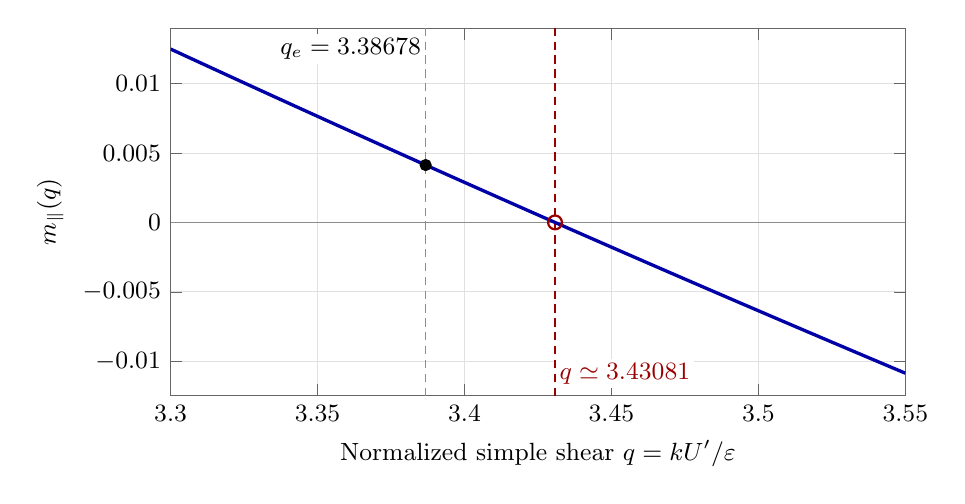
\begin{tikzpicture}
\begin{axis}[
 width=0.90\linewidth,height=6.25cm,
 xmin=3.30,xmax=3.55,ymin=-0.0125,ymax=0.0140,
 xlabel={Normalized simple shear $q=kU'/\varepsilon$},
 ylabel={$m_{\parallel}(q)$},
 xtick={3.30,3.35,3.40,3.45,3.50,3.55},
 ytick={-0.010,-0.005,0,0.005,0.010},
 scaled ticks=false,
 xticklabel={\pgfmathprintnumber[fixed,precision=2]{\tick}},
 yticklabel={\pgfmathprintnumber[fixed,precision=3]{\tick}},
 tick label style={font=\small},label style={font=\small},
 grid=major,grid style={draw=black!12},
 axis line style={draw=black!60},tick style={draw=black!60},
]
\addplot[black!45,thin,no marks] coordinates {(3.30,0) (3.55,0)};
\addplot[black!45,densely dashed,thin,no marks]
 coordinates {(3.386780140529,-0.0125) (3.386780140529,0.0140)};
\addplot[red!60!black,densely dashed,thin,no marks]
 coordinates {(3.430805647392,-0.0125) (3.430805647392,0.0140)};
\addplot[blue!65!black,very thick,no marks] coordinates {
    (3.300000000000,0.012499038317)
    (3.306250000000,0.011887440306)
    (3.312500000000,0.011277325416)
    (3.318750000000,0.010668687195)
    (3.325000000000,0.010061519232)
    (3.331250000000,0.009455815154)
    (3.337500000000,0.008851568628)
    (3.343750000000,0.008248773361)
    (3.350000000000,0.007647423096)
    (3.356250000000,0.007047511619)
    (3.362500000000,0.006449032749)
    (3.368750000000,0.005851980346)
    (3.375000000000,0.005256348307)
    (3.381250000000,0.004662130565)
    (3.386780140529,0.004137527847)
    (3.387500000000,0.004069321092)
    (3.393750000000,0.003477913894)
    (3.400000000000,0.002887903016)
    (3.406250000000,0.002299282538)
    (3.412500000000,0.001712046575)
    (3.418750000000,0.001126189278)
    (3.425000000000,0.000541704834)
    (3.430805647392,-0.000000000000)
    (3.431250000000,-0.000041412536)
    (3.437500000000,-0.000623168575)
    (3.443750000000,-0.001203568993)
    (3.450000000000,-0.001782619465)
    (3.456250000000,-0.002360325632)
    (3.462500000000,-0.002936693101)
    (3.468750000000,-0.003511727448)
    (3.475000000000,-0.004085434212)
    (3.481250000000,-0.004657818902)
    (3.487500000000,-0.005228886994)
    (3.493750000000,-0.005798643930)
    (3.500000000000,-0.006367095121)
    (3.506250000000,-0.006934245946)
    (3.512500000000,-0.007500101752)
    (3.518750000000,-0.008064667855)
    (3.525000000000,-0.008627949540)
    (3.531250000000,-0.009189952059)
    (3.537500000000,-0.009750680637)
    (3.543750000000,-0.010310140465)
    (3.550000000000,-0.010868336704)
};
\addplot[only marks,mark=*,mark size=2pt,black]
 coordinates {(3.386780140529,0.004137527847)};
\addplot[only marks,mark=o,mark size=2.5pt,thick,
 draw=red!60!black,fill=white]
 coordinates {(3.430805647392,0)};
\node[font=\small,anchor=north east,fill=white,inner sep=1.5pt]
 at (axis cs:3.386780140529,0.0136) {$q_e=3.38678$};
\node[font=\small,anchor=south west,text=red!60!black,
 fill=white,inner sep=1.5pt]
 at (axis cs:3.430805647392,-0.0120) {$q\simeq3.43081$};
\end{axis}
\end{tikzpicture}
\caption{Numerical diagnostic along the parallel simple-shear path.
Here $m_{\parallel}(q)$ is the minimum of
$\mathcal D_q/\nu_t^{\rm eff}$ over unit in-plane propagation vectors
and their unit divergence-free in-plane polarizations, with $k$ and
$\varepsilon$ frozen in the stress derivative. The neutral reference
$q_e$ and the numerical zero on this path are marked. The rigorous
all-direction reference bound $1/250$ and the exact negative
fixed-direction witness at $q=3.5$ are separate analytical results.
This curve does not define a certified boundary of an admissible
three-dimensional state set.}
\label{fig:wjstab-shear-path}
\end{figure}

\subsection{A separate general-three-dimensional realizability failure}

The general-three-dimensional cubic-root approximation has a different
admissibility limitation. Consider the dimensionless local gradient
specified by
\begin{equation}
 S=\operatorname{diag}(2,2,-4),\qquad
 \Omega=\begin{pmatrix}0&3\sqrt{17}/2&0\\
                    -3\sqrt{17}/2&0&0\\0&0&0\end{pmatrix}.
 \label{eq:wjstab-psd-counterexample}
\end{equation}
It is a legitimate incompressible affine velocity gradient with
$s=24$, $w=-153/2$, and $S\Omega=\Omega S$. Equation
\eqref{eq:wjstab-root} factors as
\begin{equation}
 (N-3)(N^2+6N/5+459/5)=0.
 \label{eq:wjstab-psd-root}
\end{equation}
Thus the prescribed root is $N=3$, and the full tensor law reduces
exactly to $a=-6S/(5N)$. Consequently,
\begin{equation}
 \boxed{R/k=\operatorname{diag}(-2/15,-2/15,34/15),
 \quad P/\varepsilon=48/5>0,\quad C_\mu^{\rm eff}=1/90>0.}
 \label{eq:wjstab-psd-failure}
\end{equation}
Two variances are negative. This counterexample specifically concerns
the selected three-dimensional explicit cubic-root approximation.
Solving the original implicit algebraic relation for this commuting
state would instead give $N=9$ and
$R/k=\operatorname{diag}(2/5,2/5,6/5)>0$. Replacing the root is a
different model choice and is not silently adopted here. It would also
leave the in-plane counterexample
\eqref{eq:wjstab-negative-witness} unchanged, because that case is
already exactly two-dimensional.

\subsection{A qualified state envelope and an optional reference-preserving change}

No constitutive change is needed to obtain
\eqref{eq:wjstab-certified} at the neutral reference. For terrain
applications, however, the original law cannot be assigned an
unrestricted ellipticity or realizability guarantee. A meaningful
qualification must specify an operating state set, positive lower
bounds for $k,\varepsilon$, and independent checks of the full stress
eigenvalues and the incompressible principal form throughout that set.
A successful coefficient-frozen implicit solve tests neither property.

If a constitutive intervention is required, a mathematically transparent
\emph{optional} reference-preserving regularization is
\begin{equation}
 R_{\rm reg}=R-\gamma(\boldsymbol x)
       [A+A^T-A_{\rm ref}-A_{\rm ref}^T],\qquad\gamma\geq0,
 \label{eq:wjstab-optional-regularization}
\end{equation}
where $A_{\rm ref}(\boldsymbol x)$ is a prescribed incompressible
reference gradient and $\gamma$ is fixed independently of the evolving
local gradient. If a verified lower bound on a declared state envelope
is $\mathcal D\geq\underline d(\boldsymbol x)
|\boldsymbol a|^2|\boldsymbol\xi|^2$, then
\begin{equation}
 \mathcal D_{\rm reg}=\mathcal D+
           \gamma|\boldsymbol a|^2|\boldsymbol\xi|^2,
 \qquad
 \gamma\geq\max\{0,d_{\rm target}-\underline d\},
 \quad d_{\rm target}>0
 \label{eq:wjstab-regularization-bound}
\end{equation}
is sufficient for that envelope. The coefficient has viscosity units.
The added stress vanishes at $A=A_{\rm ref}$, preserving its reference
stress, production, and traction. A continuation of the prescribed
reference gradient over curved terrain must be declared; no curved
equilibrium follows from the notation alone.

This is a deliberate modification of the off-reference constitutive
law. It does not by itself preserve covariance positivity, the
nonnegative-production theorem \eqref{eq:wjstab-production}, or an
absolute energy-dissipation inequality, because the imposed reference
strain contributes work. Use exactly the modified stress in momentum,
$P_{\rm reg}=-R_{\rm reg}:A$, and interface traction. An adaptive
$\gamma(A)$ adds the derivative
$D\gamma[H](A+A^T-A_{\rm ref}-A_{\rm ref}^T)$ to the tangent and
cannot be assessed by \eqref{eq:wjstab-regularization-bound} alone.
No envelope, value of $\gamma$, or globally repaired closure is selected
by the present equilibrium construction.

\subsection{Consequences for numerical qualification}

The mathematical status is therefore specific: the neutral reference
has a proved positive incompressible velocity principal bound; nearby
admissible parallel-shear states can lose forward diffusion; and the
chosen three-dimensional root approximation can also lose covariance
realizability in other states. Smaller time steps, relaxation, or a
positive implicit Laplacian with a fully compensating explicit stress
do not change these continuum properties. A resolution-dependent
filter must be assessed as part of its own effective operator.
Pressure--normal-stress balance, wall-source positivity, conservative
interface work, and the discrete equilibrium test remain independent
requirements. Any claims about a completed numerical implementation
must report which of these tests were actually passed and the state
range covered.

\section{A reproducible flat example and implementation gates}
\label{sec:wj-wall-example}

Choose $\nu=1.5\times10^{-5}\,\mathrm{m^2\,s^{-1}}$,
$u_*=0.5\,\mathrm{m\,s^{-1}}$, $H=1\,\mathrm m$,
$h=0.1\,\mathrm m$ and $z_m=H/2$, with endpoint sampling and the
calibrated coefficients. Independent evaluation gives
\begin{table}[htbp]
\centering\small
\begin{tabular}{@{}lll@{}}
\toprule
Quantity & Value & Units\\
\midrule
$K_0$ & $0.8466950351$ & $\mathrm{m^2\,s^{-2}}$\\
$b$ & $-330.8452338634$ & $1$\\
$z_v$ & $-0.0053932759$ & $\mathrm m$\\
$a$ & $0.1909589318$ & $\mathrm{m\,s^{-1}}$\\
$J_0(H)$ & $27.3022037551$ & $\mathrm{s\,m^{-1}}$\\
$J_2(H)$ & $4984.4563763332$ & $\mathrm{s^2\,m^{-3}}$\\
$A_e$ & $0.3272955050$ & $\mathrm{m^3\,s^{-3}}$\\
$\mathcal P_0$ & $1.7017148068$ & $\mathrm{m^3\,s^{-3}}$\\
$\Lambda$ & $5.1993222671$ & $1$\\
$z_c$ & $0.0150057433$ & $\mathrm m$\\
$U_{H,0}$ & $6.8255509388$ & $\mathrm{m\,s^{-1}}$\\
$z_0$ & $0.0054420488$ & $\mathrm m$\\
\bottomrule
\end{tabular}
\caption{Calibrated EP-AWF reference with positive molecular viscosity.}
\label{tab:ep-reference}
\end{table}
The gate exceeds $1+\ln2$. The interface power is
$1.7063877346915544\,\mathrm{m^3\,s^{-3}}$; molecular dissipation is
$0.004672927852812337\,\mathrm{m^3\,s^{-3}}$ and the remainder equals
$\mathcal P_0$. Hence $\nu$ has not been set to zero inside the wall law.

For shifted Legendre tests $\phi_n(z)=P_n(2z/H-1)$, split quadrature
of the unredistributed reference source gives the moments
\begin{equation}
 \begin{gathered}
 \left\{\int_0^H\phi_n(p_{A,0}-E_c)\,dz\right\}_{n=0}^4\\
 =\{0,-0.01397974167,0.03142774719,-0.04928955372,0.06586613310\}
 \ \mathrm{m^3\,s^{-3}}.
 \end{gathered}
\end{equation}
The zero displayed mean is accurate to $6\times10^{-17}$ in the
independent calculation. The EP source vanishes pointwise, so all these
moments are zero when the same reference production is used. The
positivity amendment is exactly inactive on this constant reference
for every declared $\theta,\delta\in(0,1)$.

The wall identities do not guarantee preservation of a polynomial
projection of outer $\ln z$ and $1/z$. Qualification must separately
test the complete spatial residual, algebraic constraints, common
interface fluxes, pressure normal traction and the actual timestep map
with consistent history. Keep $H,z_m$ and physical sampling fixed under
polynomial refinement; study $H$ dependence separately. Split quadrature
at all active viscosity, forcing and dissipation breakpoints, and verify
the metric budget independently. A dual source load is
$B_Q^TW_J\bm s_Q$, not a coefficient field or physical sample vector;
an interface that integrates its input must not receive an already
integrated load without the required conversion. No native solver,
global realizability, discrete positivity or long-time terrain stability
is claimed by these continuum derivations.

\subsection{Original-cutoff imbalance and the budget variant}
For the same calibrated coefficients and matching data,
$z_{\varepsilon,A}=7.7608310134\times10^{-5}\,\mathrm m$ and
$\int_0^H E_A\,dz=3.4247665028\,\mathrm{m^3\,s^{-3}}$.
The original molecular-cutoff loss is therefore different from the
required $1.7017148068\,\mathrm{m^3\,s^{-3}}$ budget. The new
plateau is $E_c(0)=21.81134911\,\mathrm{m^2\,s^{-3}}$, rather than
$E_A(0)=4217.27395412\,\mathrm{m^2\,s^{-3}}$.

The independent budget-cutoff construction keeps this $E_c$ and removes
the prescribed EP redistribution. Its exact inner reference is
\begin{equation}
 k_{w,0}^{\rm B}(z)=K_0-\int_z^H\frac{Q_c(s)}{D_{k,w}(s)}\,ds.
 \label{eq:budget-reference-comparison}
\end{equation}
The integral budget gives zero ordinary diffusive flux at both endpoints;
the local source is balanced by diffusion in every weak test moment.
Here $d=\nu-az_v=0.0010448941983\,\mathrm{m^2\,s^{-1}}>2\nu$,
which yields $Q_c<0$ and $k_{w,0}^{\rm B}>K_0$ inside the layer.
The values at $z=0$, $0.1$ and $0.5\,\mathrm m$ are respectively
$1.8887084080$, $0.9072068354$ and $0.8495674195\,\mathrm{m^2\,s^{-2}}$.
The separate standalone appendix supplies the derivation, closed
primitive, positivity proof and conservative completion of this variant.

For both flat references, the isotropic auxiliary tensor has eigenvalues
$2k_w/3$ and $2k_w/3\pm\nu_{t,A}U_{w,0}'$. Because
$k_w\geq K_0=q_eu_*^2$ and $\nu_{t,A}U_{w,0}'<u_*^2$,
its smallest eigenvalue exceeds $(2q_e/3-1)u_*^2>0$.
This is reference realizability of the auxiliary covariance; general
evolving states require a separate check.

\subsection{Metric and optional-positivity checks}
For $J(r)=(1+0.2r)(1-0.1r)$ with $r$ in metres, the reference metric
budget is $1.7302621335\,\mathrm{m^3\,s^{-3}}$ and its unique cutoff
is $r_c=0.01503619183\,\mathrm m$. Independent split integration
reproduces the budget to roundoff. This is a normal-tube kernel check,
not a terrain-flow equilibrium.
The supplied wall script also exercises the inactive, redistributed
and attenuated regimes of the sampled-$K$ amendment at $\chi=0$, an
intermediate weight and $\chi=1$. It checks common budgets, bounded
rates and consistent dependent traces. These tests concern the
analytical operators rather than a native high-order time integrator.

\section{Limits, interpretation and model choices}
\label{sec:limits}
\subsection{Finite molecular viscosity in the two equation domains}
The preceding reference is exact for a composite model whose outer
equations deliberately omit molecular transport. If molecular terms
were restored in the outer momentum and dissipation equations while
all reference fields were retained, their additional residuals would be
\begin{equation}
 \nu U_0''=-\frac{\nu u_*}{\kappa_e z^2},\qquad
 \nu\eps_0''=\frac{2\nu u_*^3}{\kappa_e z^3}.
 \label{eq:finite-nu-outer-residuals}
\end{equation}
Moreover, $\nu U_0'-R_{xz,0}$ would cease to be constant. The molecular
term in the outer $k$ equation is zero for constant $k_0$, but that
does not remove the other residuals. Their smallness when
$\nu/(\kappa_e u_*z)\ll1$ is an asymptotic statement, not an exact
finite-Reynolds-number identity.

In contrast, setting $\nu=0$ in the AWF would change its no-slip
reconstruction, virtual intercept, production budget, original cutoff,
and mechanical-energy balance. The subtraction $\nu J_2$ in
\cref{eq:wj-wall-budget} is required even if it is numerically small.
For $0<z_v<H$, the molecular segment is essential for a finite
no-slip resistance. For $z_v<0$, finite wall turbulent viscosity does
not justify discarding the physical molecular part.

The composite velocity has continuous value and total traction at $H$,
with a permissible derivative jump. It is logarithmic only in the outer
region. Numerical ground no slip does not assert that the modeled
rough-wall $k(0)$ is the microscopic viscous-sublayer value. These
choices are part of the wall model's physical interpretation.

\subsection{What is calibrated and what still needs validation}
The exact outer constants, wall coefficient calibration, cutoff budget,
and normal-pressure balance are algebraic requirements of the stated
reference. They do not calibrate the empirical roughness/intercept
relation anew. In particular, $h$, $z_0$, $H$ and a velocity offset
cannot all be prescribed independently after the momentum anchor is
fixed. Any inverse roughness calibration must report which quantity
was changed and whether the cutoff gate still holds.

Neutrality alone does not imply local equilibrium over a hill, in a
wake, or through an imposed pressure gradient. The reference-production
kernel is an identified counterfactual state, and the current mean
production remains in the actual transport equation. A spatial
transition from EP to baseline can itself generate a developing
solution because the two wall operators differ. No globally stationary
logarithm is claimed through that transition. Terrain predictions,
separation and recovery therefore require physical validation after
the mathematical and implementation gates pass.

\section{Optional remedies: operator identity and qualified scope}
\label{sec:remedy-scope}
\subsection{Variants that must remain identifiable}
The default reference uses the unmodified outer explicit WJ stress,
the calibrated auxiliary wall law, and the EP redistribution. Additional
robustness changes must be separately recorded. Table~\ref{tab:variants}
states their distinct roles. Combining modifications does not combine
their individual guarantees automatically.

\begin{table}[htbp]
\centering\small
\begin{tabularx}{\textwidth}{@{}p{0.24\textwidth}XX@{}}
\toprule
Variant & Preserved property & Remaining limitation\\
\midrule
Unmodified outer explicit WJ law
& Exact flat reference and proved positive reference principal bound
& Nearby shear can lose forward diffusion; some 3D states are unrealizable.\\
Calibrated EP-AWF
& Constant inner $k$; all reference test moments and layer budget
& Sampled destruction can deplete local $k$ away from the reference.\\
Budget-cutoff AWF
& Same outer reference; nonconstant inner $k$ balances local defect
& Reference positivity is conditional; evolving positivity is separate.\\
Capped sampled-$K$ remedy
& Exact reference on its inactive plateau; bounded destruction rate
& Severe depletion reduces the loss budget and outer $\eps$ trace.\\
Reference-centered extra stress
& Reference unchanged; specified principal bound on a qualified envelope
& Covariance, production sign and energy require new checks.\\
Discrete residual correction
& Stored projected target, if all algebraic constraints already hold
& A modified discrete scheme; conservation and consistency need verification.\\
\bottomrule
\end{tabularx}
\caption{Separate operator choices. Only the unmodified outer law and
the declared EP wall construction define the default reference.}
\label{tab:variants}
\end{table}

\subsection{A root change and a covariance intervention are separate}
One optional general-three-dimensional alternative is to determine $N$
from the exact implicit algebraic relation
\begin{equation}
 N-c_1'-\frac94\frac{\mathcal P(N)}{\eps}=0,
 \qquad \mathcal P(N)=-\eps\,\bm a(N):\bm S,
 \label{eq:implicit-3d-alternative}
\end{equation}
using the complete tensor coefficients. This is a distinct constitutive
selection, requiring its own branch continuation and derivatives. The
commuting example in \cref{eq:wjstab-psd-counterexample} then uses $N=9$
and has positive covariance. That observation is neither a global
uniqueness nor a global realizability theorem for
\eqref{eq:implicit-3d-alternative}. It leaves the exactly planar
negative-diffusion witness unchanged.

A separate covariance safeguard could blend or project
$2I/3+\bm a$ into the positive-semidefinite trace-two cone, with an
identity neighborhood of the reference. Such an intervention preserves
reference values only if it is exactly inactive there, and preserves
the reference tangent only if its derivative is also the identity
there. Away from that neighborhood, changing eigenvalues changes
production, traction and the velocity-gradient tangent. A projection
can be nonsmooth at eigenvalue ties and active bounds. Its full tangent,
energy exchange and interaction with any added incremental viscosity
must be re-evaluated. No undocumented clipping is part of this note.

\subsection{Same stress, same fluxes, same inputs}
Every changed outer stress must enter both momentum and
$\mathcal P=-\bm R:\nabla\bm U$, as well as the interface normal
and tangential traction. Otherwise mean-to-turbulent energy exchange
does not cancel. Likewise, every wall dissipation amendment must
regenerate the dependent profile and the single outer trace. Equal-input
comparisons hold $K,H,h,\nu$, matching data, physical sampling and
coefficient conventions fixed. Comparisons between independently
evolved solutions need not agree downstream after differing histories.


\section{A bounded remedy for nonlocal sampled-\texorpdfstring{$K$}{K} destruction}
\label{sec:wj-wall-positivity}

A positive prescribed dissipation is not a positivity theorem for
transported inner $k$. At $\chi=0$, a smooth locally flat zero of $k$
away from the positive endpoint sample can have zero advection, diffusion
and production, while $E_A(K)>0$. Then $\partial_tk=-E_A(K)<0$.
This is a continuum source defect, independent of polynomial undershoots.
The following replacement remains active on zero-$\chi$ baseline rays.

On each admissible ray define the common metric budget
\begin{equation}
 \mathcal B_{\rm pre}=\int_0^HJE_{\rm pre}\,dr
 =\int_0^HJD_{\rm pre}\,dr>0.
 \label{eq:wj-wall-common-budget}
\end{equation}
Choose fixed $0<\theta<1$ and $0<\delta<1$, and set
\begin{equation}
 \omega_k=\min\{1,k/(\theta K)\},\qquad
 b_k=\mathcal B_{\rm pre}^{-1}\int_0^HJD_{\rm pre}\omega_k\,dr,
 \qquad m_k=\max(b_k,\delta),\qquad \lambda_k=b_k/m_k.
 \label{eq:wj-wall-positive-weights}
\end{equation}
The limiter is defined on nonnegative $k$ and is one on an open
neighborhood of the constant reference $k/K=1$. A smooth alternative
must retain this inactive plateau and a linear bound near zero.
The normalized destruction, actual dependent dissipation and total
redistribution are
\begin{equation}
 \boxed{D_+=D_{\rm pre}\omega_k/m_k,\qquad
 E_+=\lambda_kE_{\rm pre},\qquad
 C_+=E_+-D_+,\qquad S_{k,w}^+=P_A-D_+.}
 \label{eq:wj-wall-positive-profiles}
\end{equation}
$C_+$ replaces the whole previous redistribution; it is not added
again to $C_{\rm pre}$.

For positive $k$,
\begin{equation}
 0\leq D_+/k\leq D_{\rm pre}/(\delta\theta K).
 \label{eq:wj-wall-positive-rate}
\end{equation}
At $k=0$, $D_+=0$ and $S_{k,w}^+=P_A\geq0$. With regular solutions,
positive diffusivity, bounded admissible coefficients and compatible
nonnegative boundary data, this supplies the source quasi-positivity
condition needed at a first zero. The isotropic production contribution
from weak discrete divergence also vanishes at $k=0$, but this does not
justify dropping it in an otherwise inconsistent energy discretization.
No positivity theorem for the full coupled high-order discretization,
outer turbulence equations or inner covariance follows from this result.

The exact integral identities are
\begin{equation}
 \boxed{\int_0^HJD_+\,dr=\int_0^HJE_+\,dr
 =\lambda_k\mathcal B_{\rm pre},\qquad
 \int_0^HJC_+\,dr=0.}
 \label{eq:wj-wall-positive-budget}
\end{equation}
There are three distinct regimes. If $\omega_k=1$ everywhere, then
$b_k=m_k=\lambda_k=1$ and every pre-amendment field is recovered
pointwise. Thus both the reference and every existing directional
derivative on this plateau are unchanged. If the limiter is active but
$b_k\geq\delta$, the original integrated loss and dissipation trace
are retained, while destruction is moved away from depleted points.
If $b_k<\delta$, the loss is reduced by $b_k/\delta$ to keep the
destruction rate bounded; the dependent dissipation and its trace
must decrease by the same factor.

This last concession cannot generally be avoided. A uniformly bounded
local rate $D\leq a_{\max}k$ implies
$\int JD\,dr\leq a_{\max}\int Jk\,dr$ and therefore cannot sustain
a fixed positive loss as available layer energy tends to zero.
Normalization by $b_k$ without a cap trades this budget issue for an
unbounded rate. The middle regime may increase destruction where
$\omega_k=1$ through its factor $1/b_k$; this is intentional raywise
redistribution, not a pointwise reduction everywhere.

The conservative gradient flux is
\begin{equation}
 \bm j_+=\frac{\bm n}{J(r)}\int_0^rJ(s)C_+(s)\,ds,
 \qquad \nabla\cdot\bm j_+=C_+,\qquad
 \bm j_+(0)=\bm j_+(H)=0.
 \label{eq:wj-wall-positive-flux}
\end{equation}
Use physical scalar flux $\bm U k-D_k\nabla k-\bm j_+$ with source
$P_A-E_+$, or assemble source $P_A-D_+$ with ordinary diffusion;
these are alternative representations. The shared interface flux is
unchanged because $\bm j_+$ vanishes there.

With the same production exchanged between the inner mean-flow and
turbulent-energy equations, their sum obeys
\begin{equation}
 \begin{aligned}
 \partial_t\left(\tfrac12|\bm U|^2+k\right)
 +\nabla\cdot\left[\bm U\left(\tfrac12|\bm U|^2+k\right)
 -\mathsf T_w\bm U-D_k\nabla k-\bm j_+\right]
 =-\tfrac\nu2\mathsf S_w:\mathsf S_w-E_++\bm U\cdot\bm f.
 \end{aligned}
 \label{eq:wj-wall-positive-energy}
\end{equation}
Shared traction, velocity and scalar flux cancel internal interface
work in the global budget. The raywise turbulent loss is
$\lambda_k\mathcal B_{\rm pre}$; molecular loss and roughness-force
work remain explicit. This accounting identity is not a perturbation
stability or global-existence result.

The actual dependent trace is necessarily
\begin{equation}
 \boxed{\varepsilon_o(H)=E_+(H)=\lambda_kE_{\rm pre}(H).}
 \label{eq:wj-wall-positive-trace}
\end{equation}
For continuous endpoint-sampled $k$ with $K>0$ and $D_{\rm pre}(H)>0$,
one has $b_k>0$ for each regular state; nevertheless $b_k$ can approach
zero as the positive support contracts. A uniform positive lower bound
for the outer dissipation trace is not proved. The original high-Re
closure contains ratios involving $k$ and $\varepsilon$; approaching
their degeneracy requires a separately qualified continuation or a
declared admissibility stop. An undisclosed dissipation floor is not
part of this construction.
This continuous argument is not automatically inherited by quadrature:
if the endpoint is absent from the source quadrature, all sampled
destruction weights can vanish even while $k(H)>0$. Positive quadrature
including $H$ prevents that exact zero at fixed resolution, but does not
provide a uniform lower bound under increasing degree or depletion.

At $\chi=0$ the precise positivity-adapted calibrated baseline is
\begin{equation}
 E_{\rm pre}=D_{\rm pre}=E_A,\qquad
 S_{k,w}^+=P_A-E_A\omega_k/m_k,\qquad
 E_+=\lambda_kE_A,\qquad C_+=E_A(b_k-\omega_k)/m_k.
 \label{eq:wj-wall-positive-baseline}
\end{equation}
The positivity redistribution may be nonzero even when the equilibrium
correction is zero. Disabling it over the hill would restore the failed
sampled sink. The pre-amendment calibrated baseline is recovered only on
the inactive limiter plateau. Recompute the normalization for each
baseline comparison because $D_{\rm pre}$ depends on $\chi$.

The support distinction is explicit in
$E_+=E_A+\chi(E_c-E_A)+(\lambda_k-1)E_{\rm pre}$.
Only the middle term must vanish on equilibrium-correction baseline
faces. The positivity attenuation must remain permitted there.
Trace differentiation must also include $E_{\rm pre}\nabla\lambda_k$.
With fixed geometry, state derivatives include
$\delta(k/K)=(\delta k-(k/K)\delta K)/K$, the derivative of
$D_{\rm pre}$, and the quotient-rule derivative of $b_k$.
The branch changes at $k/K=\theta$ and $b_k=\delta$ require declared
one-sided, semismooth or smooth-plateau treatment.

For frozen nonnegative production and rate, the local reaction update
$k^{n+1}=(k^n+\Delta t P_A)/(1+\Delta t D_+/k)$ is nonnegative.
It is only a source-step statement. Stage-consistent ray normalization,
advection, diffusion, projection and interface updates still require
verification. Compute both common budgets with the same positive metric
quadrature used in assembly; otherwise even plateau inactivity can be
lost through mismatched quadrature. Recompute $K$, coefficients, limiter,
cutoff and outer trace after any operation changing $k_h$.


\section{Implementation and validation programme}
\label{sec:validation}
The supplied computations verify analytical kernels, exact algebraic
certificates and a specified numerical reference. They do not constitute
an implementation in a production flow solver. The following sequence
distinguishes evidence that is available from work still required.

\subsection{G0--G2: close the model and verify local operators}
\begin{description}[style=nextline,leftmargin=2.6em]
\item[G0: operator specification.]
Record the tensor convention, full 3D or planar formula, cubic or
implicit $N$ root, $\eps$ convention, fixed scalar coefficient, exact
equilibrium constants, wall coefficients, roughness law, sampling,
matching geometry, pressure representation, and all selected amendments.
All operators must use one configuration. The formulas in this note
provide this specification for the default variant.
\item[G1: constitutive checks.]
Verify simple-shear stress, production and covariance; differentiate
the entire stress law; reproduce the exact reference certificate and
both failure examples. Use full all-direction qualifications on any
claimed operating envelope. The accompanying exact-arithmetic and
complex-step script completes the stated local checks, not an envelope
qualification for a particular terrain computation.
\item[G2: scalar wall kernels.]
Verify both viscosity branches, all momentum integrals, forcing
derivatives, traction signs, energy balance, cutoff gates, and zero
integral of each redistribution. Verify all retained modal loads and
the limiting cases $h=0$, $\chi=0$, $\chi=1$ without evaluating an
inactive invalid cutoff. The supplied flat example and curved budget
checks are reproducible kernel evidence; an implementation must repeat
them through its own assembly APIs.
\end{description}

\subsection{G3--G5: geometry, interface and discrete preservation}
\begin{description}[style=nextline,leftmargin=2.6em]
\item[G3: geometry and conservation.]
Test a flat patch, a curved normal tube and a variable-height interface.
Verify geometric stretches, physical-volume quadrature, constant-field
identities, curvature shear, normal pressure, matching measures and
normal mass flux. Check cancellation of each common internal momentum
and scalar flux, including traction work. Local $J>0$ is not a global
ray-intersection test.
\item[G4: assembled stationary residual.]
Define the projected target and evaluate continuity, momentum, $k$,
outer $\eps$, algebraic traces and all interface rows before iteration.
Refine polynomial order and quadrature independently at fixed physical
$H,z_m$. If a stored defect correction is selected, test the original
and corrected operators separately and audit its balance and consistency.
\item[G5: full timestep fixed point.]
Start all multistep histories on the same target and execute the actual
pressure, turbulence, wall reconstruction, projection and limiting
stages. Measure a single step's defect and accumulated drift.
Distinguish spatial error, pressure splitting, nonlinear tolerance
and time-integration error. A vanishing continuous source does not
make every stage stationary.
\end{description}

\subsection{G6--G8: admissibility, long-time response and terrain}
\begin{description}[style=nextline,leftmargin=2.6em]
\item[G6: positivity and admissibility.]
Exercise a depleted interior field with positive endpoint sample, both
normalization regimes of the capped remedy, and active/inactive switch
boundaries. Check the actual outer dissipation trace and admissible
ratios after every stage. Use a separately justified high-order
positivity treatment if needed; a nodal minimum alone does not exclude
between-node negativity. Record covariance and principal-symbol
margins independently of scalar minima.
\item[G7: long-time and perturbation tests.]
First retain the flat reference for many flow-through times, then add
controlled perturbations with multiple directions and wavelengths.
Measure kinetic-energy transfer, dissipation, pressure compatibility,
outer constitutive margins and limiter activity. A wavelength-dependent
failure must be distinguished from a transient physical growth or
iteration failure. Test a declared envelope, not a single converged
reference.
\item[G8: physical terrain validation.]
Only after the mathematical and discrete gates pass, compare speed-up,
normal stresses, turbulent transport, separation and reattachment with
appropriate independent measurements or trusted resolved reference
data. Report roughness and matching-height sensitivity, transition
locations, model amendments and numerical convergence. An exact inlet
does not validate off-equilibrium predictions.
\end{description}

The remaining implementation choices include switch thresholds,
positivity parameters, admissible state envelopes, optional outer
regularization, geometry treatment, trace spaces and pressure-stage
coupling. They must be selected for a stated application rather than
represented as already validated constants.

\appendix
\section{Closed AWF integrals with molecular viscosity retained}
\label{app:integrals}
\subsection{Viscosity segments and momentum}
Split the layer at any active point among $z_v$, $h$, the original
cutoff and the budget cutoff. On a molecular segment $D_A=\nu$,
\begin{equation}
 \int\frac{dz}{D_A}=\frac z\nu,\quad
 \int\frac{dz}{D_A^2}=\frac z{\nu^2},\quad
 \int\frac{z-h}{D_A}\,dz=\frac{(z-h)^2}{2\nu}
 \quad(z>h).
 \label{eq:integrals-molecular}
\end{equation}
The turbulent production is zero on this segment. On an active
linear segment let $D_A=d+az>0$, where $d=\nu-az_v$ need not be
positive if the segment begins at a positive $z_v$. With $y=d+az$,
definite primitives between points $z_1,z_2$ on the same segment are
\begin{equation}
 \begin{aligned}
 \int_{z_1}^{z_2}\frac{dz}{D_A}
 &=\frac1a\ln\frac{y_2}{y_1},\\
 \int_{z_1}^{z_2}\frac{dz}{D_A^2}
 &=\frac1a\left(\frac1{y_1}-\frac1{y_2}\right),\\
 \int_{z_1}^{z_2}\frac{z-h}{D_A}\,dz
 &=\frac{z_2-z_1}{a}
  -\frac{d+ah}{a^2}\ln\frac{y_2}{y_1}quad(z_1\geq h).
 \end{aligned}
 \label{eq:integrals-linear}
\end{equation}
No logarithm of a nonpositive extrapolated $d$ is required; use the
positive endpoint viscosities. Summing the appropriate segments gives
$J_0,J_1,J_2$ and all partial-height versions. Stable small-increment
evaluations can use $\log(1+x)$ and direct positive production
integration near cancellation.

\subsection{Production primitive for signed vector forcing}
On any active linear segment, write the shear flux as
$\bm T(z)=\bm p+\bm qz$; below $h$, $\bm q=0$ and
$\bm p=\bm t_A$, while above $h$, $\bm q=\bm F$ and
$\bm p=\bm t_A-h\bm F$.
Set $\bm f=\bm q/a$ and $\bm e=\bm p-d\bm q/a$, so
$\bm T=\bm e+\bm f y$. Then
\begin{equation}
 \begin{aligned}
 \int P_A\,dz=\frac1a\bigg[
 &|\bm f|^2\left(\frac{y^2}{2}-\nu y\right)
 +2\bm e\cdot\bm f\left(y-\nu\ln y\right)\\
 &+|\bm e|^2\left(\ln y+\frac\nu y\right)\bigg]+\mathrm{constant}.
 \end{aligned}
 \label{eq:production-primitive}
\end{equation}
Only logarithmic differences occur in definite integrals; their
arguments are dimensionless ratios. The formula follows by expanding
$(y-\nu)|\bm e+\bm f y|^2/y^2$ and using $dz=dy/a$.
It retains the signed traction and vector cross term, while the
production itself is nonnegative. Multiplying a scalar component's
production by a component count is not equivalent to this vector law.

For $0<c\leq H$, the common dissipation integral is
$A_e[1+\ln(H/c)]$. Its metric counterpart is
\cref{eq:wj-wall-metric-budget-explicit}; on general admissible geometry
use the positive physical-volume quadrature and the strictly monotone
root equation. The same quadrature defines the normalized positivity
budgets used by a discrete wall kernel.


\section{Exact all-direction reference certificate}
\label{app:wjstab-certificate}

This appendix proves \eqref{eq:wjstab-certified} using only the
reference tangent \eqref{eq:wjstab-tangent} and rational arithmetic.
Flatten a gradient matrix in row-major Cartesian order and let $M$ be
the symmetric matrix representing $H:\mathcal LH$. Its extension
outside the trace-free subspace is irrelevant to the following
calculation. The principal minors
\begin{equation}
 m_{xy}=H_{xx}H_{yy}-H_{xy}H_{yx},\quad
 m_{xz}=H_{xx}H_{zz}-H_{xz}H_{zx},\quad
 m_{yz}=H_{yy}H_{zz}-H_{yz}H_{zy}
 \label{eq:wjstab-minors}
\end{equation}
all vanish for $H=\boldsymbol a\otimes\boldsymbol\xi$. Define
\begin{equation}
 \mathcal Q(H)=H:\mathcal LH
 +\frac{289}{100}(m_{xy}+m_{yz})+\frac{57}{50}m_{xz}
 -\frac1{250}\|H\|_F^2.
 \label{eq:wjstab-proof-form}
\end{equation}
It suffices to prove $\mathcal Q(H)>0$ for every nonzero trace-free
matrix. This is a stronger finite-matrix statement than is needed for
the incompressible rank-one set.

Use the following invertible coordinates on the trace-free subspace:
\begin{equation}
 H=\sqrt{143}(t_1E_{xy}+t_2E_{xz}+t_3E_{yx}+t_5E_{zx})
       +t_4E_{yz}+t_6E_{zy}
       +t_7(E_{xx}-E_{zz})+t_8(E_{yy}-E_{zz}).
 \label{eq:wjstab-proof-coordinates}
\end{equation}
The radical scaling is only a change of coordinates and makes every
coefficient of $\mathcal Q$ rational. Reorder the coordinates as
$(t_1,t_3,t_4,t_6)$ and $(t_2,t_5,t_7,t_8)$. The resulting matrix is
block diagonal, with blocks
\begin{equation}
 K_1=\begin{pmatrix}
 35607/250&143/700&0&155/56\\
 143/700&945373/3500&-155/56&0\\
 0&-155/56&249/250&1/700\\
 155/56&0&1/700&6611/3500
 \end{pmatrix},
 \label{eq:wjstab-proof-block1}
\end{equation}
\begin{equation}
 K_2=\begin{pmatrix}
 2902757/300250&4310449/120100&6290/1201&3145/1201\\
 4310449/120100&67252757/300250&22310/1201&11155/1201\\
 6290/1201&22310/1201&713/250&713/500\\
 3145/1201&11155/1201&713/500&228793/71500
 \end{pmatrix}.
 \label{eq:wjstab-proof-block2}
\end{equation}
Their unpivoted exact $LDL^T$ diagonal pivots are, respectively,
\begin{align}
 \operatorname{diag}(D_1)=\bigg(&\frac{35607}{250},
 \frac{3295566703}{12201000},
 \frac{3188912170563}{3295566703000},
 \frac{609851247}{332332000}\bigg),
 \label{eq:wjstab-proof-pivots1}\\
 \operatorname{diag}(D_2)=\bigg(&\frac{2902757}{300250},
 \frac{2212408252197}{24379099000},
 \frac{3616758816461}{553102063049250},
 \frac{355627}{143000}\bigg).
 \label{eq:wjstab-proof-pivots2}
\end{align}
Every displayed numerator and denominator is positive; hence
$K_1\succ0$, $K_2\succ0$, and $\mathcal Q$ is positive definite on
the trace-free subspace. For an incompressible rank-one matrix,
$\operatorname{tr}H=\boldsymbol a\cdot\boldsymbol\xi=0$,
$m_{xy}=m_{xz}=m_{yz}=0$, and
$\|H\|_F^2=|\boldsymbol a|^2|\boldsymbol\xi|^2$. Substitution into
\eqref{eq:wjstab-proof-form} proves the stated lower bound.
The rational pivots are factorization quantities, not physical acoustic
eigenvalues.

The accompanying self-contained script
\texttt{wj\_stability\_checks.py} reconstructs this matrix from the
complete reference tangent and verifies the factorization in exact
arithmetic. It also compares that tangent with complex-step
differentiation of the full three-dimensional explicit stress,
reproduces the rigorous sign of
\eqref{eq:wjstab-negative-witness}, and evaluates the general
three-dimensional covariance counterexample. Its separately labeled
direction optimizations are floating-point diagnostics and are not used
to establish the certificate.


\section{Executable numerical verification}
\label{app:executable}
The following Python programs are included verbatim so this source is
self-contained. Copies are supplied as \texttt{wj\_awf\_checks.py} and
\texttt{wj\_stability\_checks.py}. They require Python 3, NumPy, SciPy
and SymPy. No external datasets are read. The wall program writes a
JSON report and a table fragment beside itself. These are kernel and
constitutive verifications; they do not implement a flow solver.

\subsection{Wall references, budgets, weak moments and positivity amendment}
\begin{lstlisting}[style=py]
#!/usr/bin/env python3
"""Independent checks for the WJ EP and budget-cutoff AWF references.

All dimensional AWF quantities retain molecular viscosity.  This evaluates
continuum formulas; it is not a finite-volume or spectral/hp solver test.
"""
from __future__ import annotations

import json
import math
from pathlib import Path

import numpy as np
from scipy.integrate import quad
from scipy.optimize import brentq
from scipy.special import spence

HERE = Path(__file__).resolve().parent
nu, ustar, H, h = 1.5e-5, 0.5, 1.0, 0.1
c1, c2, sigmak, sigmaeps = 1.8, 5.0 / 9.0, 1.0, 1.3
ce1, ce2 = 1.44, 1.82
Ne = 9.0 * c1 / 4.0
Cstar = (0.6 * Ne - 1.0) / Ne**2
qe = 1.0 / math.sqrt(Cstar)
kappae = math.sqrt(sigmaeps * (ce2 - ce1) * math.sqrt(Cstar))
K = qe * ustar**2
t0 = ustar**2
Aeps = ustar**3 / kappae
c_mu_w = Cstar
c_l_w = kappae * qe**1.5
alpha = c_mu_w * c_l_w
a = alpha * math.sqrt(K)
hstar = h * math.sqrt(K) / nu
ratio = hstar / 70.0
m = max(0.5 - 0.4 * ratio**0.7, 1.0 - 0.79 * ratio**(-0.28))
b = 10.7 * (1.0 - ratio**m)
zv = nu * b / math.sqrt(K)
d = nu - a * zv


def D(z: float) -> float:
    return nu + a * max(z - zv, 0.0)


def nut(z: float) -> float:
    return D(z) - nu


def p0(z: float) -> float:
    return t0**2 * nut(z) / D(z)**2


def J0(z: float) -> float:
    return math.log1p(a * z / d) / a


def J2(z: float) -> float:
    return (1.0 / d - 1.0 / D(z)) / a


Pquad = quad(p0, 0.0, H, epsabs=2e-13, epsrel=2e-13)[0]
Pclosed = t0**2 * (J0(H) - nu * J2(H))
Lambda = Pclosed / Aeps
zc = H * math.exp(1.0 - Lambda)


def Ew(z: float, cutoff: float = zc) -> float:
    return Aeps / max(z, cutoff)


def Rc(z: float) -> float:
    return z / zc if z <= zc else 1.0 + math.log(z / zc)


def Q(z: float) -> float:
    return Aeps * (Rc(z) - math.log1p(a * z / d)
                   + nu * (1.0 / d - 1.0 / D(z)))


def integrate_split(fun, z0: float = 0.0, z1: float = H) -> float:
    return quad(fun, z0, z1, points=[zc] if z0 < zc < z1 else None,
                epsabs=2e-13, epsrel=2e-13, limit=200)[0]


def kw(z: float) -> float:
    return K - integrate_split(lambda s: Q(s) / D(s), z, H)


zetac = a * zc / d
zetaH = a * H / d
beta = nu / d


def F_lower(zeta: float) -> float:
    log = math.log1p(zeta)
    return ((zeta - log) / zetac - 0.5 * log**2
            + beta * (log + 1.0 / (1.0 + zeta) - 1.0))


def G_upper(zeta: float) -> float:
    log = math.log1p(zeta)
    # scipy.special.spence(1+zeta) = Li_2(-zeta) on the real branch.
    return ((1.0 + math.log(zeta / zetac) + beta) * log
            + float(spence(1.0 + zeta)) - 0.5 * log**2
            + beta / (1.0 + zeta))


def F_primitive(zeta: float) -> float:
    return (F_lower(zeta) if zeta <= zetac else
            F_lower(zetac) + G_upper(zeta) - G_upper(zetac))


def kw_closed(z: float) -> float:
    return K + Aeps / a * (F_primitive(a * z / d) - F_primitive(zetaH))


def tau_turb(z: float) -> float:
    return t0 * nut(z) / D(z)


def min_covariance_eigenvalue(z: float) -> float:
    return 2.0 * kw(z) / 3.0 - abs(tau_turb(z))


cutoff_root = brentq(
    lambda c: integrate_split(lambda z: Ew(z, c)) - Pquad,
    H * 1e-5, H, xtol=1e-14,
)
production_equals_sink_at = brentq(lambda z: Ew(z) - p0(z), 0.0, zc)
z0c = H * math.exp(-a * J0(H))
UH = t0 * J0(H)
z_nodes = sorted(set([0.0, zc, 0.01, 0.1, 0.5, H]))
profiles = [
    {"z_m": z, "k_m2_s2": kw(z), "Q_m3_s3": Q(z),
     "P_m2_s3": p0(z), "E_m2_s3": Ew(z),
     "lambda_min_R_m2_s2": min_covariance_eigenvalue(z)}
    for z in z_nodes
]

# Integration-by-parts residuals use independent source quadrature and the
# analytic first integral Q; no k-value interpolation enters these checks.
weak_residuals = {}
for n in range(6):
    phi = lambda z, n=n: (z / H)**n
    dphi = lambda z, n=n: 0.0 if n == 0 else n / H * (z / H)**(n - 1)
    diffusion = -integrate_split(lambda z: Q(z) * dphi(z))
    source = integrate_split(lambda z: (p0(z) - Ew(z)) * phi(z))
    weak_residuals[str(n)] = diffusion + source

# A curved normal tube is only a metric-budget check, not a terrain equilibrium.
kappa1, kappa2 = 0.2, -0.1
J = lambda r: (1.0 + kappa1 * r) * (1.0 + kappa2 * r)
PJ = quad(lambda r: J(r) * p0(r), 0.0, H, epsabs=1e-13)[0]
def curved_budget(c: float) -> float:
    return Aeps * (1.0 + math.log(H / c)
                   + (kappa1 + kappa2) * (H - c / 2.0)
                   + kappa1 * kappa2 * (H**2 / 2.0 - c**2 / 6.0))
curved_cutoff = brentq(lambda c: curved_budget(c) - PJ, H * 1e-5, H,
                       xtol=1e-14)
curved_budget_quad = quad(lambda r: J(r) * Ew(r, curved_cutoff), 0.0, H,
                         points=[curved_cutoff], epsabs=1e-13)[0]

# Conditional positivity amendment: use the same quadrature-defined sink
# budget in numerator and denominator, so the inactive plateau is exact.
theta, delta, power = 0.5, 0.1, 20
B_sink = integrate_split(Ew)
b_reference = integrate_split(lambda z: Ew(z) * 1.0) / B_sink
omega_depleted = lambda z: min(1.0, (z / H)**power / theta)
z_switch = H * theta**(1.0 / power)
limiter_integral = lambda f: quad(
    f, 0.0, H, points=sorted([zc, z_switch]),
    epsabs=2e-13, epsrel=2e-13, limit=200
)[0]
b_depleted = limiter_integral(lambda z: Ew(z) * omega_depleted(z)) / B_sink
m_depleted = max(b_depleted, delta)
lambda_depleted = b_depleted / m_depleted
D_positive = lambda z: Ew(z) * omega_depleted(z) / m_depleted
E_positive = lambda z: lambda_depleted * Ew(z)
C_positive = lambda z: E_positive(z) - D_positive(z)

checks = {
    "calibrated_a_error": a - kappae * ustar,
    "calibrated_A_error": Aeps - t0**2 / a,
    "outer_epsilon_compatibility": ce1 - ce2 + kappae**2 / (sigmaeps * math.sqrt(Cstar)),
    "production_closed_minus_quadrature": Pclosed - Pquad,
    "budget_E_minus_P": integrate_split(Ew) - Pquad,
    "cutoff_closed_minus_numerical_root_m": zc - cutoff_root,
    "Q_H": Q(H),
    "max_k_primitive_minus_quadrature": max(abs(kw_closed(z) - kw(z)) for z in z_nodes),
    "momentum_interface_traction_error": D(H) * (t0 / D(H)) - t0,
    "dissipation_trace_error": Ew(H) - Aeps / H,
    "pressure_normal_traction_error": (-K / Ne) + 2.0 * K / 3.0 - (2.0 / 3.0 - 1.0 / Ne) * K,
    "mechanical_energy_error": t0 * UH - nu * t0**2 * J2(H) - Pquad,
    "weak_residuals_n0_to_5": weak_residuals,
    "rough_gate_pass": Lambda >= 1.0,
    "interior_half_height_gate_pass": Lambda >= 1.0 + math.log(2.0),
    "sufficient_positivity_condition_pass": zv <= 0.0 and d >= 2.0 * nu,
    "minimum_inner_covariance_eigenvalue_at_H": min_covariance_eigenvalue(H),
    "analytic_covariance_lower_bound": (2.0 * qe / 3.0 - 1.0) * t0,
    "curved_budget_quadrature_error": curved_budget_quad - PJ,
    "outer_simple_shear_cubic_error": (
        Ne**3 - 9.0 / 4.0 * (c1 - 1.0) * Ne**2
        - 7.0 / 20.0 * qe**2 * Ne
        - 9.0 / 4.0 * (c1 - 1.0) * qe**2
    ),
    "limiter_reference_inactivity_error": b_reference - 1.0,
    "limiter_destruction_budget_error": limiter_integral(D_positive) - lambda_depleted * B_sink,
    "limiter_redistribution_integral_error": limiter_integral(C_positive),
    "limiter_dependent_trace_error": E_positive(H) - lambda_depleted * Aeps / H,
    "limiter_zero_destruction_error": D_positive(0.0),
}
for key, value in checks.items():
    if key.endswith("pass"):
        assert value, (key, value)
    elif key in {"minimum_inner_covariance_eigenvalue_at_H", "analytic_covariance_lower_bound"}:
        assert value > 0.0, (key, value)
    elif key == "weak_residuals_n0_to_5":
        assert max(abs(x) for x in value.values()) < 1e-10, value
    else:
        assert abs(value) < 1e-10, (key, value)

values = {
    "nu": nu, "ustar": ustar, "H": H, "h": h, "Cstar": Cstar,
    "qe": qe, "kappae": kappae, "Ne": Ne, "K": K,
    "c_mu_w": c_mu_w, "c_l_w": c_l_w, "alpha": alpha, "a": a,
    "hstar": hstar, "m": m, "b": b, "zv": zv, "d": d,
    "Aeps": Aeps, "P0_integral": Pquad, "Lambda": Lambda, "zc": zc,
    "UH": UH, "z0c": z0c, "k_wall": kw(0.0), "k_0p1": kw(0.1),
    "k_0p5": kw(0.5), "p_wall": p0(0.0), "E_wall": Ew(0.0),
    "source_zero_m": production_equals_sink_at,
    "pressure_offset_m2_s2": -K / Ne,
    "viscous_mean_dissipation_integral": nu * t0**2 * J2(H),
    "curved_kappa1": kappa1, "curved_kappa2": kappa2,
    "curved_cutoff": curved_cutoff, "curved_reference_P": PJ,
    "first_zero_derivative_at_H_over_4": -Ew(H / 4.0),
    "limiter_theta": theta, "limiter_delta": delta,
    "limiter_depleted_power": power, "limiter_depleted_b": b_depleted,
    "limiter_depleted_lambda": lambda_depleted,
    "limiter_depleted_loss": lambda_depleted * B_sink,
    "limiter_depleted_epsilon_trace": E_positive(H),
}
payload = {"values": values, "profiles": profiles, "checks": checks}
(HERE / "quantitative_checks.json").write_text(json.dumps(payload, indent=2) + "\n")

table_rows = [
    (r"$K$", K, r"$\mathrm{m^2\,s^{-2}}$"),
    (r"$z_v$", zv, r"$\mathrm{m}$"),
    (r"$a$", a, r"$\mathrm{m\,s^{-1}}$"),
    (r"$d$", d, r"$\mathrm{m^2\,s^{-1}}$"),
    (r"$\Lambda$", Lambda, r"$1$"),
    (r"$\mathcal P_0$", Pquad, r"$\mathrm{m^3\,s^{-3}}$"),
    (r"$z_c$", zc, r"$\mathrm{m}$"),
    (r"$U_{H,0}$", UH, r"$\mathrm{m\,s^{-1}}$"),
    (r"$z_{0,w}$", z0c, r"$\mathrm{m}$"),
    (r"$k_{w,0}(0)$", kw(0.0), r"$\mathrm{m^2\,s^{-2}}$"),
    (r"$k_{w,0}(0.1\,\mathrm m)$", kw(0.1), r"$\mathrm{m^2\,s^{-2}}$"),
    (r"$k_{w,0}(0.5\,\mathrm m)$", kw(0.5), r"$\mathrm{m^2\,s^{-2}}$"),
    (r"$\min_{[0,H]}\lambda_{\min}(R_w)$", min_covariance_eigenvalue(H), r"$\mathrm{m^2\,s^{-2}}$"),
]
table = [r"\begin{table}[htbp]", r"\centering\small",
         r"\begin{tabular}{@{}lll@{}}", r"\toprule",
         r"Quantity & Value & Units\\", r"\midrule"]
table.extend(f"{name} & ${value:.10f}$ & {units}\\\\" for name, value, units in table_rows)
table += [r"\bottomrule", r"\end{tabular}",
          r"\caption{Budget-cutoff WJ wall-layer reference.  All entries retain the stated molecular viscosity; these are analytical reference values, not flow-solver validation.}",
          r"\label{ba:table-reference}", r"\end{table}"]
(HERE / "reference_table.tex").write_text("\n".join(table) + "\n")
print(json.dumps({"values": values, "checks": checks}, indent=2))

# EP modal balance, signed forced momentum, and the capped sampled-K remedy.
# These tests share the physical constants above but evaluate budgets with
# independent split quadrature. They are analytical-kernel checks only.
from scipy.special import eval_legendre

ep_moments = [integrate_split(
    lambda z, n=n: eval_legendre(n, 2*z/H-1)*(p0(z)-Ew(z)))
    for n in range(5)]
assert abs(ep_moments[0]) < 1e-12
assert max(abs(x) for x in ep_moments[1:]) > 1e-2
# At unit EP weight the net source is assembled as P_A - p0.
assert max(abs(integrate_split(
    lambda z, n=n: eval_legendre(n, 2*z/H-1)*(p0(z)-p0(z))))
    for n in range(5)) == 0.0

J1H = quad(lambda z: max(z-h, 0.0)/D(z), 0, H, points=[h])[0]
Ftest, UHtest = 0.4, 0.7*UH
tA = (UHtest-Ftest*J1H)/J0(H)
TH = tA + Ftest*(H-h)
def Uforced(z):
    j1 = quad(lambda s: max(s-h, 0.0)/D(s), 0, z,
              points=[h] if z>h else None)[0]
    return tA*J0(z)+Ftest*j1
def shear_forced(z):
    return (tA+Ftest*max(z-h, 0.0))/D(z)
forced_energy = (TH*UHtest
    - quad(lambda z: D(z)*shear_forced(z)**2, 0,H,points=[h])[0]
    - Ftest*quad(Uforced,h,H)[0])
assert abs(Uforced(0)) < 1e-12
assert abs(Uforced(H)-UHtest) < 1e-11
assert abs(forced_energy) < 1e-10

theta, delta = 0.5, 0.2
zEA = 2*c_l_w*nu/math.sqrt(K)
EA = lambda z: Aeps/max(z,zEA)
metric = lambda z: 1+0.05*z
PJlim = quad(lambda z: metric(z)*p0(z),0,H,epsabs=1e-12)[0]
def metric_budget(c):
    return Aeps*(1+math.log(H/c)+0.05*(H-c/2))
zc_lim = brentq(lambda c: metric_budget(c)-PJlim,1e-7,H)
EC = lambda z: Aeps/max(z,zc_lim)
def qi(f):
    return quad(f,0,H,points=[zEA,zc_lim,0.25,0.5,0.9],
                epsabs=2e-11,epsrel=2e-11,limit=500)[0]
limiter_checks = []
for chi in (0.0,0.35,1.0):
    epre = lambda z: (1-chi)*EA(z)+chi*EC(z)
    dpre = lambda z: (1-chi)*EA(z)+chi*p0(z)
    budget = qi(lambda z: metric(z)*epre(z))
    assert abs(budget-qi(lambda z: metric(z)*dpre(z))) < 2e-10
    for name, ratio in (
        ('inactive',lambda z: 1.0),
        ('redistributed',lambda z: 0.30+0.70*z/H),
        ('attenuated',lambda z: (z/H)**80)):
        omega = lambda z: min(1.0,ratio(z)/theta)
        bk = qi(lambda z: metric(z)*dpre(z)*omega(z))/budget
        mk, lam = max(bk,delta), bk/max(bk,delta)
        sink = lambda z: dpre(z)*omega(z)/mk
        epsp = lambda z: lam*epre(z)
        sink_budget = qi(lambda z: metric(z)*sink(z))
        eps_budget = qi(lambda z: metric(z)*epsp(z))
        assert abs(sink_budget-eps_budget) < 2e-10
        assert abs(sink_budget-lam*budget) < 2e-10
        if name=='inactive':
            assert abs(bk-1)<2e-10 and abs(lam-1)<2e-10
        if name=='attenuated':
            assert bk<delta and 0<lam<1
        for z in np.linspace(0,H,101):
            kval=K*ratio(z)
            if kval==0:
                assert sink(z)==0
            else:
                assert sink(z)/kval <= dpre(z)/(delta*theta*K)*(1+1e-12)
        limiter_checks.append(dict(chi=chi,regime=name,b=bk,attenuation=lam,
            budget_error=sink_budget-eps_budget,
            trace=epsp(H)))

payload['ep_checks'] = dict(
    unredistributed_legendre_moments=ep_moments,
    forced_energy_error=forced_energy,
    forced_ground_traction=tA,forced_interface_traction=TH,
    molecular_cutoff=zEA,
    baseline_dissipation_integral=qi(EA),
    limiter_cases=limiter_checks)
(HERE/'quantitative_checks.json').write_text(json.dumps(payload,indent=2)+'\n')
print('EP higher-mode, forced-power and capped-positivity checks: PASS')
print(json.dumps(payload['ep_checks'],indent=2))

\end{lstlisting}

\subsection{Exact reference certificate and adverse constitutive states}
The exact rational factorization, complex-step tangent comparison and
two counterexamples are checked before the separately labeled
floating-point direction diagnostics.
\begin{lstlisting}[style=py]
"""Self-contained exact reference certificate and off-reference WJ checks.
Requires Python 3, NumPy, SymPy, and SciPy. No data files are read.
The model uses the full 3D tensor basis and the explicit 2D cubic N root.
The certificate is exact rational arithmetic; optimized values are diagnostic.
"""
import numpy as np
import sympy as sp
from scipy.optimize import differential_evolution
from itertools import combinations

F=sp.Rational; r=sp.sqrt(143); Cstar=F(572,6561); qstar=1/sp.sqrt(Cstar)
cp=1.8

def constitutive(B, Nguess=None):
    """Dimensionless anisotropy a, effective coefficient, cubic N."""
    S=(B+B.T)/2; O=(B-B.T)/2; I=np.eye(3)
    s=np.trace(S@S); w=np.trace(O@O); iv=np.trace(S@O@O)
    if Nguess is None:
        rr=np.roots([1,-cp,-2.7*s-2*w,2*cp*w])
        N=max(z.real for z in rr if abs(z.imag)<1e-9)
    else:
        N=Nguess
    for _ in range(12):
        f=N**3-cp*N*N-(2.7*s+2*w)*N+2*cp*w
        df=3*N*N-2*cp*N-2.7*s-2*w
        d=f/df; N-=d
        if abs(d)<1e-14: break
    Q=(5/6)*(N*N-2*w)*(2*N*N-w)
    b1=-N*(2*N*N-7*w)/Q; b3=-12*iv/(N*Q)
    b4=-2*(N*N-2*w)/Q; b6=-6*N/Q; b9=6/Q
    a=(b1*S+b3*(O@O-w*I/3)+b4*(S@O-O@S)
       +b6*(S@O@O+O@O@S-(2/3)*iv*I)
       +b9*(O@S@O@O-O@O@S@O))
    return a,-.5*(b1+w*b6),N

def numeric_tangent(B):
    _,C,N=constitutive(B)
    cols=[]
    for h in np.eye(9):
        aa,_,_=constitutive(B.astype(complex)+1e-30j*h.reshape(3,3),N)
        cols.append(-aa.imag.ravel()/(1e-30*C))
    L=np.column_stack(cols)
    return L,(L+L.T)/2

# Exact derivative of -R divided by nu_eff at the reference; row-major order.
L=sp.Matrix([
 [F(386,143),0,-40*r/1201,0,0,0,10300*r/171743,0,F(100,143)],
 [0,1,0,F(53,28),0,-10*r/143,0,-125*r/4004,0],
 [10*r/143,0,F(86,1201),0,0,0,F(1886,1201),0,-10*r/143],
 [0,1,0,F(53,28),0,-10*r/143,0,-125*r/4004,0],
 [F(775,2002),0,0,0,F(53,14),0,0,0,F(775,2002)],
 [0,10*r/143,0,125*r/4004,0,1,0,F(53,28),0],
 [10*r/143,0,F(86,1201),0,0,0,F(1886,1201),0,-10*r/143],
 [0,10*r/143,0,125*r/4004,0,1,0,F(53,28),0],
 [F(100,143),0,40*r/1201,0,0,0,-10300*r/171743,0,F(386,143)]])
M=(L+L.T)/2
minor_matrices=[]
for i,j in combinations(range(3),2):
    for t,u in combinations(range(3),2):
        V=sp.zeros(9)
        V[3*i+t,3*j+u]+=F(1,2); V[3*j+u,3*i+t]+=F(1,2)
        V[3*i+u,3*j+t]-=F(1,2); V[3*j+t,3*i+u]-=F(1,2)
        minor_matrices.append(V)
weights=[F(289,100),0,0,0,F(57,50),0,0,0,F(289,100)]
Z=[]
for i,j in [(0,1),(0,2),(1,0),(1,2),(2,0),(2,1)]:
    H=sp.zeros(3); H[i,j]=r if i==0 or j==0 else 1
    Z.append(sp.Matrix(list(H)))
Z.extend([sp.Matrix(list(sp.diag(1,0,-1))),sp.Matrix(list(sp.diag(0,1,-1)))])
Z=sp.Matrix.hstack(*Z)
K=sp.simplify(Z.T*(M+sum((w*V for w,V in zip(weights,minor_matrices)),sp.zeros(9))
                         -F(1,250)*sp.eye(9))*Z)
assert all(v.is_Rational for v in K)
ll,dd=K.LDLdecomposition(hermitian=False)
pivots=list(dd.diagonal())
assert all(d>0 for d in pivots)
assert K==ll*dd*ll.T
print('EXACT CERTIFICATE: D >= nu_eff/250 on all incompressible rank-one increments.')
print('Exact positive LDL pivots:',[str(d) for d in pivots])

B=np.zeros((3,3)); B[0,2]=float(qstar)
Ln,Mn=numeric_tangent(B)
err=np.max(np.abs(Ln-np.array(L,dtype=float)))
assert err<1e-12
print('Full tensor complex-step / exact tangent maximum error:',err)

def direction_minimum(M):
    def projected(angles, return_data=False):
        t,p=angles
        n=np.array([np.sin(t)*np.cos(p),np.sin(t)*np.sin(p),np.cos(t)])
        u=np.array([np.cos(t)*np.cos(p),np.cos(t)*np.sin(p),-np.sin(t)])
        v=np.array([-np.sin(p),np.cos(p),0])
        J=np.column_stack([np.outer(u,n).ravel(),np.outer(v,n).ravel()])
        e=np.linalg.eigvalsh(J.T@M@J)
        return (e,n) if return_data else e[0]
    opt=differential_evolution(projected,[(0,np.pi),(0,2*np.pi)],seed=832,tol=1e-10)
    return opt.fun,projected(opt.x,True)[1]

print('NUMERICAL reference optimized minimum / nu_eff and normal:',direction_minimum(Mn))

# Rigorous sign of one fixed adverse direction at q=7/2.
N=sp.symbols('N'); p=80*N**3-144*N**2-343*N-1764
lo=F(413,100); hi=F(414,100)
assert p.subs(N,lo)<0 and p.subs(N,hi)>0
# p has exactly one positive root by its coefficient signs.
g=37338352*N*N-156626001*N+59032897
assert g.subs(N,lo)>0 and sp.diff(g,N).subs(N,lo)>0
assert (240*N*N-288*N-343).subs(N,lo)>0
witness=-g/(6250*N*(4*N*N+49)*(240*N*N-288*N-343))
print('EXACT COUNTEREXAMPLE: q=7/2, unique positive N in (4.13,4.14), D/nu_eff<0.')
B[0,2]=3.5; a,C,Nn=constitutive(B); _,Mn=numeric_tangent(B)
n=np.array([1.,0,-7])/np.sqrt(50); u=np.array([7.,0,1])/np.sqrt(50)
h=np.outer(u,n).ravel(); value=h@Mn@h
assert abs(value-float(witness.subs(N,Nn)))<1e-12
assert value<0 and np.linalg.eigvalsh(a+2*np.eye(3)/3).min()>0
print('q=3.5 fixed-direction value / nu_eff:',value)
print('q=3.5 covariance eigenvalues / k:',np.linalg.eigvalsh(a+2*np.eye(3)/3))
print('q=3.5 production / epsilon:',-np.sum(a*B))
print('NUMERICAL q=3.5 optimized minimum / nu_eff:',direction_minimum(Mn))

# Exactly specified general-3D cubic-surrogate realizability counterexample.
S=np.diag([2.,2.,-4.]); O=np.zeros((3,3))
O[0,1]=1.5*np.sqrt(17); O[1,0]=-O[0,1]
aa,CC,NN=constitutive(S+O)
assert abs(NN-3)<1e-12
assert np.max(np.abs(aa+2*np.eye(3)/3-np.diag([-2/15,-2/15,34/15])))<1e-12
print('EXACT 3D cubic-surrogate covariance/k = diag(-2/15,-2/15,34/15).')
print('Production/epsilon = 48/5, C_mu_eff = 1/90; covariance is not PSD.')
print('PASS: reference certificate and off-reference counterexamples verified.')

\end{lstlisting}

\begin{thebibliography}{9}
\bibitem{WJ2000}
S.~Wallin and A.~V.~Johansson,
``An explicit algebraic Reynolds stress model for incompressible and
compressible turbulent flows,''
\emph{Journal of Fluid Mechanics} \textbf{403}, 89--132 (2000).
\href{https://doi.org/10.1017/S0022112099007004}{doi:10.1017/S0022112099007004}.

\bibitem{Baungaard2022}
M.~Baungaard, S.~Wallin, M.~P.~van der Laan and M.~Kelly,
``Wind turbine wake simulation with explicit algebraic Reynolds stress
modeling,'' \emph{Wind Energy Science} \textbf{7}, 1975--2002 (2022).
\href{https://doi.org/10.5194/wes-7-1975-2022}{doi:10.5194/wes-7-1975-2022}.

\bibitem{SCI2006}
K.~Suga, T.~J.~Craft and H.~Iacovides,
``An analytical wall-function for turbulent flows and heat transfer over
rough walls,'' \emph{International Journal of Heat and Fluid Flow}
\textbf{27}(5), 852--866 (2006).
\href{https://doi.org/10.1016/j.ijheatfluidflow.2006.03.011}{doi:10.1016/j.ijheatfluidflow.2006.03.011}.
\end{thebibliography}

\end{document}
